% --- (1) Einseitiges Dokument ---
\documentclass[a4paper,12pt]{scrreprt}
\usepackage{listings}
\usepackage{amsmath}
% Grafiken im Fließtext
\usepackage{floatflt}
\usepackage[pdftex]{graphicx}
% tikz => Diagramme
\usepackage{tikz}
% Grafiken mit Hilfe von [H] an der definierten Stelle platzieren
\usepackage{here}
% UML-Diagramme mit Hilfe von tikz
\usepackage[
% school,
% simplified
]{pgf-umlcd}
\RequirePackage[utf8]{inputenc}
% CKL: Dieses LaTeX-Dokument ist für einen einseitgen Druck ausgelegt.
% CKL: Dafür sorgen, dass die Fußnotennummerierung nicht mit jedem Kapitel neu beginnt
\usepackage{remreset}
\makeatletter
\@removefromreset{footnote}{chapter}
\makeatother

% ==========[ Einstellungen laden ]==========

\input{wissenschaftlich_arbeiten_latex.settings}


\begin{document}


% ==========[ Deckblatt mit Angaben zum Dokument ]==========

\titelSeiteDaten
{Bachelor-Thesis} % Art der Arbeit
{}
{w3l in Kooperation mit der FH Dortmund} % Name der Hochschule
{Informatik} % Fachbereichsname
{Web- und Medieninformatik} % Name des Studiengangs
{Integration von Xtext in einen \mbox{bestehenden} Softwareentwicklungsprozess} % Titel der Arbeit
{}
{}
\titelSeiteNamen
{Christopher Klein} % Name des Autors
{7078647} % Matrikel-Nummer
{Dr.-Ing. Sandra Krüger} % Name des Erstprüfers
{Prof. Dr. Heide Balzert}
{22. April 2013} % Abgabedatum

% ==========[ Schriftgroesse und Zeilenhoehe ]==========

\fontsize{12pt}{13pt}\selectfont


% ==========[ Inhaltsverzeichnis ]==========

% Gliederungstiefe des Inhaltsverzeichnisses
\setcounter{tocdepth}{1}

% Inhaltsverzeichnis
\tableofcontents

% ==========[ Beginn des eigentlichen Inhaltes ]==========

% Layout pruefen und Nummerierung anpassen
\leerSeiteInhalt


% Blocksatz aktivieren
\sloppy

\chapter{Abstrakt}
\index{Abstrakt}
In Softwareprojekten wird der Großteil des Quellcodes von Hand geschrieben, obwohl sich viele der notwendigen Artefakte aus vorhandenen Informationen automatisiert generieren ließen. Die Generierung von Quellcode reduziert die Fehleranfälligkeit innerhalb der zu entwicklenden Anwendung und sorgt dafür, dass mehr Zeit in die Implementierung der Geschäftslogik investiert werden kann.
\\
\\
In dieser Bachelorarbeit wird untersucht, wie ein bestehender Softwareentwicklungsprozess durch Automatismen verbessert werden kann. Diese Erkenntnisse bilden die Basis für die Entwicklung einer domänenspezifischen Sprache mit Hilfe des Werkzeugs Xtext. Neben der Anpassung der Xtext-Umgebung wird die Grundlage für einen Plug-in-Mechanismus geschaffen. Dieser Mechanismus erlaubt das einfache Einbinden von Generatoren, die aus dem Domänenmodell Artefakte generieren können. Auf diesen Mechanismus setzen die beiden implementierten Generatoren auf: Aus dem gegebenen Domänenmodell erzeugen sie daraus einerseits Mockups und andererseits eine Function Point-Analyse.
\\
\\
Die Nutzung von Xtext hat den Softwareentwicklungsprozess entschieden verbessert: Die Planung von zukünftigen Projekten ist nun durch die gegebene Möglichkeit einer Function Point-Analyse einfacher geworden. Während der Phase des Requirement Engineerings wurden die generierten Mockups bereits in ersten Projekten zu Demonstrationszwecken gezeigt. Besonders der einfache Plug-in-Mechanismus und die implementierten Erweiterungen für Xtext haben für eine deutliche Verbesserung des Prozesses gesorgt. Auf dieser Grundlage wurden nach kurzer Zeit weitere Generatoren entwickelt, die Quellcode für verschiedene Programmiersprachen und Anwendungsgebiete erzeugen. Die Entwickler können sich nun mehr auf die Implementierung der Geschäftslogik konzentrieren.
\chapter*{Abstract}
\index{Abstract}
In software projects most of the source code is written by hand although most of the required artifacts could be automatically generated through existing information. The generation of source codes reduces the error-proneness inside the application to be developed and ensures that more time can be invested into the development of the business logic.
\\
\\
This dissertation examines how an existing software development process can be improved through use of suitable automatisms. This knowledge forms the base for the development of a domain specific language through use of the tool Xtext. Besides the adaption of the Xtext environment a basis for a plug-in mechnism is created. This mechanism provides the easy integration of generators. The generators use the domain model for generating artifacts. Both of the implemented generators use this mechanism: By using the given domain model they generate on the one hand a mockup and on the other hand a function point analysis.
\\
\\
The usage of Xtext definitely improved the software development process: the planning for future projects is now easier with help of the function point analysis. The generated mockups have been already used in the phase of requirement engineering. Particularly the easy-to-use plug-in mechanism and the implemented extensions for Xtext showed a clearly improvement of the process. On this basis more generators for generating source code for different programming languages and use cases have been developed in a short time. Developers can now more focus on the business logic.
\chapter{Einleitung}
\index{Einleitung}
"Write Code That Writes Codes" \cite{ht2006}
lautet einer der Ratschläge aus \textit{The Pragmatic Programmers}, einem der bekanntesten Bücher der Softwareentwicklung. Die Idee besteht darin, dass sich wiederholende Programmieraufgaben durch geeignete Methoden und Techniken automatisieren lassen. Auf dieser Idee basiert der Ansatz der modellgetriebenen Entwicklung: die automatisierte Generierung von Quellcode auf Basis eines definierten Modells. Gerade mit der stetig steigenden Anzahl der Technologien ist es wichtig, dass sich die Softwareentwickler auf die jeweiligen Domänenprobleme konzentrieren können und nicht durch wiederkehrende Standardanforderungen und -aufgaben während des Entwicklungsprozesses Zeit verlieren.
Neben proprietären Werkzeugen zur Code-Generierung existieren auch freie Alternativen.

\section{Aufgabenstellung}
Das Ziel dieser Bachelorthesis soll es sein, dass ein bestehender Softwareent\-wick\-lungs\-prozess durch technische Lösungen verbessert werden soll. Der Schwerpunkt liegt dabei auf der automatischen Generierung von Code-Fragmenten mit Hilfe des Xtext-Frameworks. 
Die resultierenden Code-Fragmente können dabei unterschiedlicher Natur sein, z.B. Quellcode für C\#, PHP oder Java, Dokumentation, automatische Analysen oder Dateien mit SQL-Anweisungen
\\
\\
Das im Rahmen dieser Bachelorarbeit entstehende Eclipse Plug-in soll dabei so entwickelt werden, dass neue Generatoren für Code-Fragmente einfach integriert werden können.
\section{Motivation}
Auslöser für diese Bachelor-Arbeit ist ein abgeschlossenes Software-Projekt gewesen, in dem bereits Xtext im kleinen Rahmen verwendet wurde.
Die dabei erstellte domänenspezifische Sprache (\textit{Domain Specific Language}, \textit{DSL}) beschrieb die Domänen-Objekte mit ihren Attributen, die mit Hilfe von Xtext in C\#-Quellcode umgewandelt wurden.
Die DSL wurde zwar nur für grundlegende Transformationen benutzt, dennoch lag der dadurch entstandene Mehrwert auf der Hand. Es entstand eine einheitliche Basis für Dokumentation und Quellcode. Die Zeit, die für alltägliche Programmierarbeiten wie dem Implementieren von Entitäten oder der Datenzugriffsschicht anfiel, wurde auf ein Minimum verringert.
\section{Vorgehen}
Zuerst wird der Softwareentwicklungsprozess bei der NeosIT GmbH vorgestellt und mögliche Verbesserungen aufgezeigt.
Im darauffolgenden Kapitel wird die Grundidee hinter der modellgetriebenen Softwareentwicklung gezeigt und verschiedene Lö\-sungs\-an\-sätze und Produkte kurz erläutert. Als Einführung in die Arbeit mit Xtext werden im Kapitel \ref{ch:technologien} die notwendigen Technologien und Ideen vorgestellt, die dieses Werkzeug mit sich bringt.\\
Die Umsetzung der Verbesserungsvorschläge findet durch die Implementierung statt. Das Kapitel \ref{ch:realisierung} erläutert die während der Bachelorarbeit entstandenen Code-Generatoren.
Schlussendlich wird ein Fazit gezogen und Ausblick auf zukünftige Erweiterungen gegeben.
\\
\\
Während dieser Ausarbeitung gelten folgende Konventionen:
\begin{itemize}
	\item Pfadangaben und Dateinamen werden in kursiver Schrift dargestellt, z.B. \textit{src/plugin.xml}
	\item Quellcode wird in Verbatim dargestellt, z.B. \texttt{addComponent(...)}
	\item Innerhalb des Quellcodes bedeuten von rechts unten nach links oben stehende Schrägstriche am Ende der Zeile, dass der folgende Zeilenumbruch nur aus Platzgründen eingeführt worden ist. Der Quellcode steht regulär mit der nächsten Zeile zusammen in einer Zeile.
	\item Bei Verweisen auf Methoden werden die Parameterdefintionen nicht mit angegeben und durch drei Punkte \texttt{...} ersetzt
	\item Bei Verweisen auf Klassen- oder Interfacenamen wird nicht der vollqualifizierte Name angegeben, sondern nur der Instanzname. Der vollqualifizierte Name wird als Fußnote hinterlegt. Anstatt \texttt{de.ckl.rapid.RapidRuntimeModule} wird nur \texttt{RapidRuntimeModule} geschrieben.
\end{itemize}

\chapter{Ausgangssituation}
\section{Kontext}
Die Bachelorarbeit wird innerhalb des Unternehmens NeosIT GmbH in Wolfsburg ge\-schrieben. Die NeosIT ist ein mittelständisches IT-Unternehmen, dass in den Bereichen Softwareentwicklung und Systemadministration tätig ist. Zu den Kunden zählen unter anderem die Volkswagen AG und die Volkswagen Financial Service AG.\\
Neben dem Customizing bestehender Open-Source-Software wird auch Software nach Bedarf des Kundens programmiert.
Die meisten Projekte werden dabei in C\#, Java oder PHP realisiert und stehen dem Kunden als Webapplikationen innerhalb des Intra- oder Internets zur Verfügung.\\
Besondere Erfahrung haben die Mitarbeiter der NeosIT in der Entwicklung von webbasierten Management-Reporting-Systemen. Es handelt sich dabei um Software zur Auswertung von Unternehmenskennzahlen. Die Auswertung findet dabei tabellarisch oder mit Hilfe von geeigneten Charts statt. Grundlage für diese Art von Software bilden in aller Regel bereits existierende Excel-Tabellen, die in eine Webanwendung transformiert werden sollen.
\section{Aktueller Entwicklungsprozess}
Im Folgenden soll ein Einblick in den aktuell vorhandenen Softwareent\-wick\-lungs\-prozess bei der NeosIT GmbH gegeben werden. Eine detaillierte Beschreibung würde den Rahmen dieser Arbeit sprengen.
\subsection{Requirements Engineering}
In der Phase des Requirements Engineering werden die Anforderungen des Kunden aufgenommen.
Idealerweise existiert seitens des Kunden ein detailliertes Lastenheft, das alle Anforderungen enthält. Die Vergangenheit hat aber gezeigt, dass solche idealisierten Vorstellungen sich selten bewahrheiten.
Aus diesem Grund wird das Lastenheft gemeinsam durch Auftraggeber und Auftragnehmer erstellt.\\
Nachdem die groben Anforderungen an die zu erstellende Software in ersten Meetings geklärt worden ist, werden detailierte Funktionalitäten besprochen. Je nach Anforderung des Kunden werden hier bereits mögliche Konzepte zur grafischen Gestaltung der Benutzerführung vorgestellt. Die möglichen Konzepte werden dabei mit Software wie Adobe Photoshop, Gliffy oder Balsamiq umgesetzt.\\
Es hat sich dabei gezeigt, dass der frühe Einsatz von Mockups deutliche Vorteile für den weiteren Projektverlauf bietet:
\begin{itemize}
	\item Zwischen Auftraggeber/Auftragnehmer entsteht eine emotionale Beziehung zu der zu erstellenden Software. Es handelt sich nicht mehr um etwas Abstraktes, was erst in ferner Zukunft anfassbar ist. Beide Seiten werden angeregt über eine langfristige Vision nachzudenken.\\
	Die Entwickler können dabei oft aus den Äußerungen des Kunden erkennen, welche zusätzlichen Wünsche auftreten könnten und die zu erstellende Softwarearchitektur darauf abstimmen. Lässt sich beispielsweise bereits im Vorfeld erkennen, dass neben einer Weboberfläche eventuell eine mobile Anwendung benötigt wird, werden die öffentlichen Schnittstellen bereits entsprechend aufbereitet angeboten.
	\item Der Kunde kann anhand von grafischen Elementen einfacher beschreiben, wie seine internen Prozesse ablaufen. Missverständnisse zwischen Auftragnehmer und Auftraggeber können so in einer frühen Phase geklärt werden, die später zu teuren Refactoring-Maßnahmen führen würden\footnote{siehe \cite{cl2010} bzw. \cite{ebdu96}}.
	\item Die Entwickler können anhand der Ergebnisse (Anforderungen, Wünsche, Prozessabläufe) eine bessere Abschätzung zu den zu leistenden Stunden abgeben.
\end{itemize}

Im Gegensatz zu den funktionalen Anforderungen werden die nicht-funktionalen Anforderungen anhand von Formblättern aufgenommen. Hier werden messbare Größen wie z.B. gefordertes Antwortverhalten dokumentiert. Weiterhin werden unter anderem folgende Themenkomplexe abgefragt:
\begin{itemize}
	\item Gegenwärtige Situation der IT-Landschaft - wie sieht die Netzwerkinfrastruktur aus; welche IP-Bereiche existieren; kommt Nating zum Einsatz; existieren Proxy-Server; welche Mailserver existieren etc.
	\item Bereits in Planung befindliche Änderungen	der IT-Landschaft
	\item Zwingend einzusetzende Software wie z.B. DBMS, Frameworks oder Server-Applikationen inklusive der Versionen.
\end{itemize}
Die Formblätter werden in aller Regel von den zuständigen Systemadministratoren ausgefüllt.
Seitens des Auftragnehmers werden in einer virtuellen Umgebung die relevanten Systeme in einem kleinen Rahmen nachgebaut. Dabei wird vor allem auf den Einsatz von identischen Versionen geachtet: Unterschiedliche Datenbankmanagementsysteme haben von Version zu Version andere Features; die zu erstellenden Dokumentation für die Systemadministration unterscheidet sich von Betriebssystem-Version zu Betriebssystem-Version etc.
\\
Alle Anforderungen und Mockups werden im Anschluss in das unternehmensinterne Confluence-Wiki übertragen und stehen allen Mitarbeitern sowie dem Auftraggeber zur Verfügung.
Im Wiki wird ebenfalls die Endanwender- und Entwickler-Dokumentation des Projektes gepflegt.
\subsection{Analyse und Konzeptionierung}
Sobald die Anforderungen an die Software definiert worden sind, werden diese analysiert. 
Im ersten Schritt werden die Objekte innerhalb des Anforderungskatalogs identifiziert. Die Attribute der Objekte und die Beziehung zu anderen Objekten werden dokumentiert.\\
Die Ergebnisse der Analyse werden direkt in ein UML-Klassendiagramm überführt. Dies gilt später als Grundlage für das zu erstellende Datenbankmodell.
\\
Die einzusetzende Software ergibt sich einerseits aus den Anforderungen des Kunden, andererseits aus den bisher gemachten Erfahrungen der Entwickler. Die Software-Architektur basiert dann auf der eingesetzten Software. In den meisten Fällen findet aber eine strikte Trennung zwischen Datenzugriffsschicht\footnote{DAL bzw. DAO-Entwurfsmuster}, Serviceschicht und Frontend statt. Im Frontend kommt ebenfalls in den meisten Fällen das MVC-Pattern zum Einsatz.\\
Je nach Plattform werden weitere Frameworks eingegliedert. Tabelle \ref{frameworks} enthält einen Auszug der favorisierten Frameworks für C\# und Java.

\begin{table}[h]
\begin{tabular}{l|l|l}
Komponente 	& 		C\# 		&	 Java\\
\hline
Logging 	& NLog oder log4net & log4j \\
Dependency Injection & Unity oder Spring.NET & Spring oder Guice \\
MVC & ASP.NET MVC 2/3 & Spring MVC \\
Scheduling 	& Quartz.NET 		& Quartz 	\\
Messaging Queue & ActiveMQ 		& ActiveMQ 	 \\
AOP & Unity & AspectJ \\
Testing & Xunit & JUnit \\
\end{tabular}
\caption{\label{frameworks}Eingesetzte Frameworks}
\end{table}
Sobald die Software-Architektur definiert und mit dem Auftraggeber abgestimmt ist, werden die Schnittstellen zwischen den einzelnen Subsystemen definiert.
\subsection{Realisierung}
Zuerst wird das unspezifizierte Datenbankmodell auf das konkret ausgewählte DBMS übertragen. Das bedeutet, dass die DDL-Statements so erstellt werden, dass sie innerhalb des DBMS funktionieren. Je nach Datenbankmanagementsystem können sich Datentypen oder andere Optionen unterscheiden. Um zukünftige Änderungen an dem Datenbankschema einfacher handhaben zu können, werden die SQL-Statements über Tools automatisiert ausgeführt\footnote{siehe dazu https://github.com/schakko/db-migrator bzw. https://github.com/prunkstar/db-migrator.net}.
\\
\\ 
Anhand der im Vorfeld definierten Schnittstellen werden die einzelnen Komponenten von den Entwicklern programmiert. Durch eine lose Koppelung und dem Einsatz von Dependency Injection-Frameworks lässt sich noch nicht implementierte Funktionalität mit Hilfe von Mocks abbilden. Somit können mehrere Entwickler an verschiedenen Komponenten gleichzeitig arbeiten. Die Quellcodeverwaltung erfolgt dabei über Git.
Als Standard-Entwicklungsumgebung wird für Java- und PHP-Projekte Eclipse eingesetzt\footnote{Mit den Umgebungen JDT bzw. PDT}, bei C\#-Projekten kommt hingegen Visual Studio zum Einsatz.
\\
\\
In aller Regel wird ein iteratives bzw. agiles Vorgehensmodell wie Kanban oder Scrum gewählt, so dass der Kunde schnell benutzbare Software erhält. Die Qualitätssicherung geschieht dabei über die Unittest-Frameworks der einzelnen Plattformen\footnote{Xunit oder JUnit} oder mit zusätzlichen Tools\footnote{z.B. Selenium}. Die Builds werden durch einen Buildserver\footnote{TeamCity, http://www.jetbrains.com/teamcity/} automatisiert erstellt.
\section{Ist-Aufnahme bestehender Automatismen}
\label{sec:verbesserung}
Der momentane Entwicklungsprozess wird bereits durch einige Automatismen unterstützt, die folgend kurz beschrieben werden sollen.
\subsection{Generierung der Verzeichnisstruktur eines Projekts}
Zu Beginn eines Projekts wird manuell ein Projektverzeichnis angelegt, das eine standardisierte Ordnerstruktur enthält. Dieses Verzeichnis wird in das zentrale Git\footnote{Git ist eine verteilte Versionsverwaltung; siehe http://www.git-scm.com}-Repository gepusht. Jeder Entwickler arbeitet mit einer verteilten Kopie des Repositories.
\\
Die Erstellung der standardisierten Ordnerstruktur sowie das Generieren von initialen Dateien, wie z.B. README-Dateien, erfolgt momentan über ein eigenes PowerShell-Script.
Jeder Entwickler findet sich somit in neuen Projekten sofort zurecht und Vorlagen von Buildscripten können ohne Pfadanpassungen integriert werden.
\subsection{Kontinuierliche Integration}
Unter dem Begriff \emph{Kontinuierliche Integration} versteht man das automatische Erstellen der Build-Artefakte, sobald neuer Quellcode in eine Versionverwaltung eingecheckt worden ist.\\
Bei der NeosIT wird dabei TeamCity\footnote{http://www.jetbrains.com/teamcity/} eingesetzt. Diese Applikation überprüft in regelmäßigen Intervallen, ob in den Git-Repositories neuer Quellcode gepusht worden ist. Bei einer Änderung wird dieser auf einen sogenannten Buildagent ausgecheckt und das durch den Administrator definierte Buildscript gestartet. Die Buildscripte enthalten jeweils Anweisungen zum Ausführen von Unittests und zur Kompilierung. Die Projektmitglieder werden per E-Mail über Fehler innerhalb des Build- oder Testprozesses informiert.\\
Nach erfolgreichen Build- und Testphase werden die generierten Artefakte in passende ZIP- oder MSI-Pakete transformiert und stehen allen Entwicklern und den Kunden direkt zur Verfügung.
\subsection{Kontinuierliches Deployment}
Die durch den Buildserver entstandenen Artefakte werden zum Teil automatisiert auf den Test- oder Produktivsystemen ausgerollt, so dass der Benutzer sofort die Änderungen sehen kann. Unter anderem können sich in Entwicklung befindliche Kundenwebseiten automatisch ausgerollt werden.
\section{Ideen zur Verbesserung}
\label{sec:verbesserung}
Neben den bereits bestehenden Automatismen gibt es natürlich viele weitere Anwendungsfälle, die sich automatisieren und in den bestehenden Softwareentwicklungsprozess integrieren ließen. 
\subsection{Function Point-Analyse}
\label{sub:fpa}
Bei der Function Point-Analyse handelt es sich um ein algorithmisches Schätzverfahren um den benötigten Aufwand zur Umsetzung eines Softwareprojektes zu ermitteln. Die Methode ist unter anderem in der Norm ISO/IEC 20926 standardisiert. Für das Schätzverfahren werden unterschiedliche Elemente des Anforderungskatalogs gezählt und gewichtet. Die Regeln, nach denen vorgegangen wird, hat unter anderem die International Function Point User Group\footnote{IFPUG, http://www.ifpug.org} festgelegt \cite{bal2009}.
Für jedes Projekt wird eine Function Point-Analyse durchgeführt und die dabei entstandenen Ergebnisse in einer zentraler Datenbank festgehalten.\\
Durch die Formel 
$\frac{Summe\ aller\ Function\ Points}{Summe\ aller\ aufgewendeten\ Projektstunden}$ wird abgebildet, wie lange die Umsetzung eines Function Points in Stunden dauert. Es soll hier nicht verschwiegen werden, dass die Analyse nur einen groben Hinweis auf die Dauer geben kann:
\begin{itemize}
	\item Die aufgewendeten Projektstunden müssen bereinigt sein, so dass Stunden für Meetings und Abstimmungsgespräche nicht enthalten sind.
	\item Bestimmte Aufgaben lassen sich mit einer Programmiersprache oder einem eingesetzten Framework einfacher umsetzen, als mit einem anderen.
	\item Direkten Einfluss auf die aufgewendeten Stunden hat das Projektteam. Einerseits wird die Performance eines gleichbleibenden Teams mit den selben Technologien über die Zeit besser werden. Andererseits können neue Projektmitglieder die Gesamtperformance negativ oder positiv verändern. Idealerweise sollte das selbe Team mit den selben Technologien arbeiten. 
\end{itemize}
Eine automatisierte Function Point-Analyse ließe sich recht schnell mit einer verfügbaren DSL implementieren.

\subsection{Generierung eines Mockups}
\label{sub:gen_prototyp}
Während der Phase des Requirements Engineerings könnten alle funktionalen Anforderungen sofort in einer dafür vorgesehenen Beschreibungssprache aufgenommen werden.
Die dabei definierten notwendigen Attribute, Objekte und Beziehungen könnten automatisch in einen Mockup transformiert werden. Mockups sind Attrappen, die zu Präsentationszwecken gefertigt wurden und wenig bis keine Funktionalität beinhaltet.
Der generierte Mockup beinhaltet eine rudimentäre Oberfläche, die die Standardaufgaben von Software enthält, wie z.B. Einträge bearbeiten oder auflisten. Die Funktionslogik selbst ist dabei nicht implementiert. Alle Eingabefelder ergeben sich aus den Datentypen der Attribute. Der Kunde kann somit bereits während der Definition der Anforderungen sehen, wie ein Teil seiner gewünschten Anwendung aussehen könnte.\\
Zur einfachen Erzeugung eines Prototypen bietet sich eine automatische Ge\-ne\-rie\-rung mittels HTML und CSS an.  
Idealerweise kann der Anwender auswählen, in welchem Design bzw. mit welchem Stylesheet die Anwendung erzeugt werden soll. Kunden, bei denen öfter Projekte umgesetzt werden, sehen dabei den Mockup sofort im bekannten Corporate Design. 
\subsection{Generierung einer benutzbaren Ober\-flä\-che}
\label{sub:gen_gui}
Sobald die Datenzugriffsschicht und die zugehörigen Entitäten existieren, könnte eine Oberfläche automatisiert generiert werden. Bei Rails- oder ASP.NET MVC-Applikationen könnte dies über Scaffolding-Funktionalitäten der Frameworks ge\-schehen \cite{railsScaffolding}. Im Gegensatz zum Mockup würde bei diesem Automatismus Funktionslogik zur Verarbeitung und Persistierung enthalten sein. Der Aufwand zur Umsetzung eines solchen Generators ist dementsprechend höher.

\subsection{Generierung der Verzeichnisstruktur für den Quellcode}
Innerhalb des Projektverzeichnisses existiert der Ordner \textit{src/} der jedweden Quellcode enthält. Je nach eingesetzter Programmiersprache sind alle darin enthaltenen Unterverzeichnisse nach einem bestimmten Schema zu benennen. Bei Java-Projekten wird z.B. das Maven-Verzeichnislayout benutzt.
\\
Sobald die Entscheidung für eine Software-Architektur getroffen wurde, ließe sich hiermit die Verzeichnisstruktur generieren.
\subsection{Einbinden von Bibliotheken}
Bibliotheken und Frameworks werden je nach Projekt über Mechanismen wie NuGet\footnote{http://www.nuget.org}, Ivy\footnote{http://ant.apache.org/ivy/} oder Maven\footnote{http://maven.apache.org} eingebunden.
\\
Ebenfalls mit der Entscheidung für eine Software-Architektur ließen sich in den passenden Konfigurationsdateien die Standard-Bibliotheken aus Tabelle \ref{frameworks} einbinden. 
\subsection{Generierung der Dokumentation des Datenbankschemas}
Das Datenbankdiagramm mit den Tabellen und Relationen wird im bestehenden Prozess manuell in der Online-Dokumentation hinterlegt, so dass neue Entwickler einen schnellen Überblick über die Datenstruktur haben. Bei Änderungen muss dieses Diagramm und weitere Dokumentation zum Datenbankschema aktualisiert werden.
\\
Ein Ziel sollte es sein, dass bei einer Änderung der Anforderungen automatisch das Datenbankschema neu erstellt und die Dokumentation aktualisiert wird.
\subsection{Generierung von Migrationen bei Än\-de\-run\-gen am Datenbankschema}
Alle Projekte des bestehenden Softwareentwicklungsprozesses nutzen bereits das Konzept von Datenbankschema-Migrationen. 
Sobald ein Entwickler eine Änderung am Datenbankschema der Applikation vornehmen will, muss er diese Änderung in einem eigenen SQL-Script hinterlegen. Jedes SQL-Script ist für sich genommen eine eigene Migration und enthält beliebige SQL-Statements. Die Scripte werden natürlich innerhalb des Git-Repositories versioniert.\\
Mit dem Erstellen der Applikation werden vom Buildscript automatisch alle ausstehenden Migrationen auf die Datenbank angewendet.
Die Datenbanken der anderen Entwickler werden nach dem letzten Git-Pull und mit dem nächsten Build aktualisiert. Weiterhin lassen sich diese Migrationen packen und beim Kunden automatisiert einspielen.
\\
Wünschenswert ist es nun, dass bei Änderungen der funktionalen Anforderungen automatisch eine passende Migration erstellt werden würde. Beispielsweise möchte der Kunde für seine Applikation ein zusätzliches Feld namens "Nachname". Es würde automatisch eine Migration mit dem Befehl 
\begin{verbatim}
ALTER TABLE xyz ADD COLUMN nachname char(255);
\end{verbatim}
 erstellt werden.
\subsection{Generierung von Quellcode für die Datenzugriffsschicht}
\label{sub:gen_dao}
Aus dem Klassendiagramm ergibt sich direkt, welche Entitäten bzw. Transfer-Objekte erzeugt werden. Die Entitäten enthalten alle Attribute, die das Objekt besitzt. Die Persistierung erfolgt dabei über die Datenbankzugriffsschicht. Jede Entität wird über eine DAL- bzw. DAO-Klasse \cite{daoPattern} persistiert oder geladen. Jede DAO-Klasse stellt ihre Methoden über ein zugehöriges Interface bereit.
\\
Die zu erstellenden Klassen ähneln sich und nehmen bei einer manuellen Implementierung viel Zeit in Anspruch. Durch geeignete Implementierung kann zwar der Aufwand für die CRUD-Methoden reduziert werden, die Entitäts-Klassen müssen hingegen immer händisch erzeugt werden. Eine automatisierte Ge\-ne\-rie\-rung auf Basis des Klassendiagramms ist wünschenswert.
\section{Ziele}
Im Rahmen eines Kundenprojekts wurde das erste Mal Xtext zur automatischen Generierung von Code-Fragmenten genutzt\footnote{Konkret wurde die Generierung wie in Kapitel \ref{sub:gen_dao} beschrieben, vorgenommen}.\\
In der Retroperspektive des Projekts wurde beschlossen, dass Xtext als Basis für zukünftige Projekte benutzt werden soll.
Ein erster Schritt hin zur Umsetzung dieser Entscheidung ist die vorliegende Bachelorarbeit. Es geht dabei um folgende Ziele:
\begin{itemize}
	\item Es muss eine formale Sprache spezifiziert werden, die den in Kapitel
	\ref{sec:verbesserung} beschriebenen Ideen gerecht wird. Die Spezifizierung der Sprache wird mit anderen Entwicklern und deren Anforderungen an die DSL abgestimmt.
	\item Es muss ein Mechanismus geschaffen werden, mit dem auf einfache Art und Weise aus der formalen Sprache unterschiedliche Artefakttypen generiert werden können. Die Komplexität hinter Xtext und Eclipse soll dabei verborgen bleiben, so dass auch Webdesigner oder Personen ohne Programmierhintergrund die DSL nutzen und erweitern können.
	\item Es muss die Möglichkeit gegeben sein, dass der Entwickler für ein Projekt definieren kann, welche Code-Artefakte erzeugt werden sollen. Es muss also eine Konfigurationsoberfläche existieren, in der der Entwickler dediziert Generatoren aktiveren oder deaktivieren kann.\\
	\item Folgende Generatoren sollen im Rahmen der Bachelorarbeit implementiert werden:
		\begin{itemize}
			\item Die Prototypen-Generierung aus Kapitel \ref{sub:gen_prototyp} soll umgesetzt werden. Dabei wird durch HTML und CSS ein Prototyp erzeugt, der sich durch die in den DSL definierten funktionalen Anforderungen ergibt. Es soll weiterhin die Möglichkeit bestehen, dass der Entwickler das Stylesheet für einen Prototyp auswählen kann. Webdesigner müssen ohne großen Aufwand in der Lage sein, neue Stylesheets zu integrieren.
			\item Die Function Point-Analyse aus Kapitel \ref{sub:fpa} soll automatisch erzeugt werden.
		\end{itemize}
\end{itemize}
Alle weiteren Anforderungen sollen im Laufe zusätzlicher Projekt- bzw. Ab\-schluss\-ar\-bei\-ten realisiert werden. Xtext soll eine zentrale Position bei der Umsetzung neuer Softwareprojekte innerhalb der NeosIT einnehmen.
\chapter{Einführung in die Technologien}
\label{ch:technologien}
Aufgrund der Komplexität des Xtext-Frameworks ist es nötig, dass zuerst die im Rahmen dieser Thesis eingesetzten Technologien und Ideen kurz vorgestellt werden.
\section{Modelle und  Metamodelle}
Domänenspezifische Sprachen stellen Sprachelemente bereit, um später eine be\-stimm\-te Problemdomäne, zum Beispiel eine Applikation, konkret zu beschreiben.
Dabei wird für die konkrete Problemdomäne auch der Begriff \textit{Modell} benutzt.
Die verfügbaren und erlaubten Elemente des Modells werden hingegen mit Hilfe des \textit{Metamodells} definiert. Beispielsweise kann das Metamodell definieren, dass jedes Modell über Elemente vom Typ Domäne verfügen muss und dabei jede Domäne Attribute besitzen darf. Bei der objektorientierten Programmierung wäre eine Klasse das  Metamodell, eine Objektinstanz dieser Klasse hingegen das konkrete Modell.
Damit nun eine domänenspezifische Sprache, das  Metamodell, beschrieben werden kann, wird das \textit{Metametamodell} eingeführt. Diese Sprachebene stellt eine Grundmenge bereit, um beliebige Metamodelle zu definieren. Innerhalb der objektorientierten Programmierung könnten die Schlüsselwörter und genutzten Zeichen der Programmiersprache als Metametamodell angesehen werden.
Die Grafik \ref{fig:meta-meta-modell} stellt die Beziehung zwischen den drei Begrifflichkeiten noch einmal dar.

\begin{figure}[h]
	\centering
		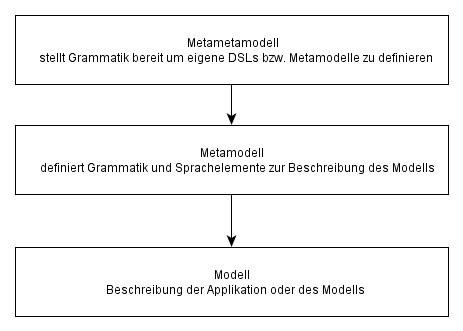
\includegraphics[width=300px]{diagramme/meta-meta-modell.png}
		\caption{Modell,  Metamodell und Metametamodell}
		\label{fig:meta-meta-modell}
\end{figure}

\section{Modellgetriebene Softwareentwicklung}
Bei der modellgetriebenen Softwareentwicklung geht es in erster Linie um das Ableiten einer Applikation aus der Implementierung einer formalen Beschreibungssprache. Die Komplexität der dahinter liegenden Programmiersprache soll durch eine Abstrahierung der Problemebene versteckt werden. Die Erhöhung der Produktivität und kürzere Entwicklungszyklen stehen dabei im Vordergrund. Die Sprache zur Beschreibung der Problemdomäne wird \textit{Domain Specific Language} (DSL) genannt \cite{mdsd}.
\\
Bei domänenspezifischen Sprachen wird zwischen internen und externen DSLs unterschieden. Interne DSLs werden in bereits bestehenden Programmiersprachen eingebettet. Dabei kann jede Programmiersprache als Host für eine interne DSL genutzt werden. Die Entwicklung solch einer DSL kann von jedem durchgeführt werden, der mit der Syntax der Host-Programmiersprache vertraut ist. Häufig wird dabei das Konzept von Fluent Interfaces zur Abbildung eingesetzt. Die Programmiersprache Scala erlaubt beispielsweise eine recht hohe Anpassungsfähigkeit der Sprache, womit sich interne DSLs mit einer bestimmten Grammatik recht einfach abbilden lassen. Durch die enge Bindung an die Host-Programmiersprache werden interne Sprache in aller Regel von Softwareentwicklern eingesetzt.
\\
Externe DSLs hingegen sind eigenständige Sprachen, deren Syntax und Sprachfeatures frei definiert werden können. Die Syntax kann so gewählt werden, dass sie auch für Endanwender ohne Kenntnisse in der Softwareentwicklung einfach und intuitiv zu bedienen sind. Neben Xtext existieren einige weitere Lösungen zum Erstellen von externen DSLs.
Kommerzielle Produkte wie beispielsweise MetaEdit erlauben eine grafische Modellierung der DSL und lassen sich seit Version 5.0 über Plug-ins in Visual Studio und Eclipse einbinden. JetBrains bietet mit MPS eine Open Source Lösung an, mit der sich DSLs innerhalb einer IDE entwickeln lassen. 
Microsoft stellte unter dem Codenamen Oslo eine Sammlung von Werkzeugen vor, um Entwicklern bei der Erstellung von DSLs und Datenbankabfragen zu unterstützen. Oslo bestand aus den den Komponeten \textit{Repository}, \textit{Quadrant} und \textit{M}. \textit{M} diente dabei der Definition von DSLs und ähnelt in Ansätzen der Syntax von ANTLR \cite{programmingLanguageM}. Quadrant war hingegen ein grafisches Tool ur Bearbeitung von Datensätzen innerhalb eines Microsoft SQL Servers \cite{quadrantOverview}. Nachdem die Entwicklung dieser Werkzeuge nicht weiter verfolgt worden ist, veröffentlichte Microsoft das Visualization and Modeling SDK mit dem sich ebenfalls DSLs entwickeln lassen, die innerhalb des Visual Studios eingesetzt werden können \cite{visualizationAndModelingSdk}. 
\section{Eclipse}
IBM begann die Entwicklung an der integrierten Entwicklungsumgebung Eclipse für Java im Jahre 1998 \cite{historyEclipse}. Durch die Veröffentlichung von Eclipse unter einer Open Source-Lizenz Ende 2001 bekamen auch andere Personen die Möglichkeit, Software auf Basis von Eclipse zu entwickeln. 
Neben den Java Development Tools entstanden zum Beispiel die PHP Development Tools zur Entwicklung von PHP-Projekten oder die Business Intelligence and Reporting Tools zur Erzeugung von Berichten.\\
Der offizielle Eclipse Marketplace enthält Anfang 2013 rund 1500\footnote{http://marketplace.eclipse.org/} ver\-öf\-fent\-lichte Plug-ins - viele weitere sind über weitere Quellen verfügbar.
Eclipse selbst ist eine Java-Applikation, die innerhalb einer JVM läuft.
Die aktuelle Eclipse-Runtime 4.2 setzt dabei auf den OSGi-Container Eclipse Equinox auf, der von der Eclipse Foundation entwickelt worden ist.
\subsection{OSGi}
Der OSGi-Container ist auf Basis der OSGi-Spezifikation entwickelt worden \cite{osgiSpec}. Die Spezifikation definiert unter anderem für so genannte Komponenten (Bundles) einen Lebenszyklus, wie er in Abbildung \ref{fig:bundlelifecycle} dargestellt ist. 
\begin{figure}[h]
	\centering
		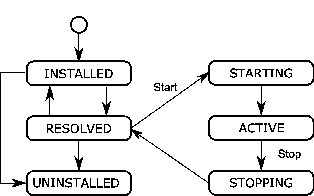
\includegraphics[width=200px]{img/bundlelifecycle.png}
		\caption{Lifecycle-Zustände für OSGi-Bundle nach \cite{osgiLifecycle}}
		\label{fig:bundlelifecycle}
\end{figure}

In Eclipse ist jedes Plug-in eine Komponente und kann somit installiert, gestartet, gestoppt und deinstalliert werden. Über eine zentrale Service-Registy wird die Schnittstelle der Komponente veröffentlicht und kann von anderen Komponenten angesprochen werden.\\
Über die Datei \textit{META-INF/MANIFEST.MF} eines Bundles wird unter anderem festgelegt, welche Klassen veröffentlicht werden und von anderen Komponenten sichtbar sind.\\
Neben der \textit{MANIFEST.MF} besitzt in Eclipse jedes Plug-in eine Datei mit dem Namen \textit{plugin.xml}, das die Erweiterbarkeit des Plug-ins definiert.
\subsection{Extension und Extension Points}
Eclipse sieht vor, dass jedes Plug-in Extension Points definieren kann. Extension Points werden anderen Plug-ins zur Verfügung gestellt, um die Funktionalität des bereitstellenden Plug-ins zu erweitern.
Sobald ein Plug-in solch einen Extension Point in Anspruch nimmt, gilt das Plug-in als eine Extension. Ein Plug-in kann beliebig viele Extension Points bereitstellen und konsumieren.\\
Welche Extension Points bereitgestellt oder genutzt werden, wird innerhalb der \textit{plugin.xml} definiert. Zusätzlich bietet die \textit{Eclipse Plug-in Development Environment} die Möglichkeit, dass diese Konfiguration mit einem grafischen Editor vorgenommen werden kann.
\\
\\
Die Eclipse Workbench stellt von Haus aus bereits viele Extension Points zur Verfügung, so dass man z.B. Menüeinträge, Eigenschaftsseiten oder Editoren hinzufügen oder ändern kann.
\subsection{Features}
Sobald mehrere Plug-ins zusammengefasst werden, spricht man in Eclipse von Features. Damit ist nur gemeint, dass die Plug-ins organisatorisch zusammen gehören. Beispielsweise könnte das Feature \textit{de.ckl.groovy.feature} eine Entwicklungsumgebung für Groovy sein und aus den einzelnen Plug-ins \textit{de.ckl.groovy.editor} und \textit{de.ckl.groovy.viewer} bestehen.
\subsection{Workbench}
In aller Regel erweitern die Plug-ins von Features die Extension Points der Workbench IDE UI. Die Workbench bietet unterschiedliche Extension Points an, z.B. um auf die Menüeinträge zuzugreifen oder neue Text-Editoren für einen bestimmten Dateityp zu registrieren.\\
Die Workbench selbst definiert unterschiedliche GUI-Elemente wie Tree-Viewer oder Editoren. Die Darstellung geschieht dabei mit Hilfe der GUI-Frameworks JFace bzw. SWT.\\
Über so genannte Perspektiven werden unterschiedliche GUI-Elemente von Plug-ins zusammengefasst. Dies ermöglicht das schnelle Wechseln zwischen un\-ter\-schied\-lichen Plug-in-Ansichten. Die Perspektive \textit{Java} zeigt z.B. standardmäßig die logische Struktur des Java-Projekts über eine Tree-View und den Java-Quellcode-Editor an. Die Perspektive \textit{Debug} deaktiviert hingegen die Tree-View und aktiviert das Plug-in zum Anzeigen des aktiven Stack Traces einer laufenden Java-Applikation.
\subsection{Projekte}
Anhand des Typs eines Projekts wird beim Laden desselben die zugehörige Perspektive initialisiert. Sobald ein neues Projekt durch die Eclipse IDE erstellt wird, wird innerhalb des Hauptverzeichnis des Projekts ein neuer Ordner \textit{.settings} und die Datei \textit{.project} erstellt.\\
Im Ordner \textit{.settings} werden projektspezifische Einstellungen von Eclipse Plug-ins gespeichert. Beispielsweise enthält die Datei \textit{.settings/org.eclipse.jdt.core.prefs} Informationen darüber, in welcher Java-Version der Quellcode vorliegt.
Die Dateien werden dabei im .properties-Format gespeichert, so dass in jeder Zeile einer solchen Datei die Einstellungen im Format \begin{verbatim}Schlüssel=Wert\end{verbatim} hinterlegt sind. 
\\
\\
Die Datei \textit{.project} enthält über eine definierte XML-Struktur Metainformationen über das Projekt, z.B. welche Natures oder Builder aktiviert worden sind \cite{projectFileDesc}.
\\
\\
Natures definieren, welche Plug-ins bzw. Features einem bestimmten Projekt zugeordnet sind \cite{projectBuildersAndNatures}. 
Eine Nature kann z.B. \textit{Java} oder \textit{Xtext} sein. 
Neben den Natures wird in der \textit{.project}-Datei hinterlegt, welche Builder existieren. Builder erzeugen, je nach Konfiguration automatisch oder manuell angesteuert, die Artefakte, die sich aus den Quellcodedateien ergeben. Der Java-Builder ruft beispielsweise für jede \textit{.java}-Datei eines Projekts den Java-Compiler auf, der wiederum den Quellcode in eine \textit{.class}-Datei kompiliert.
\\
\\
Jedem Projekt können mehrere Natures und Builder zugeordnet sein.
Das Diagramm in Abbildung \ref{fig:eclipse-beziehungen} stellt die grobe Beziehung zwischen den einzelnen Komponenten innerhalb der Eclipse-Umgebung grob dar.
\begin{figure}[h]
	\centering
		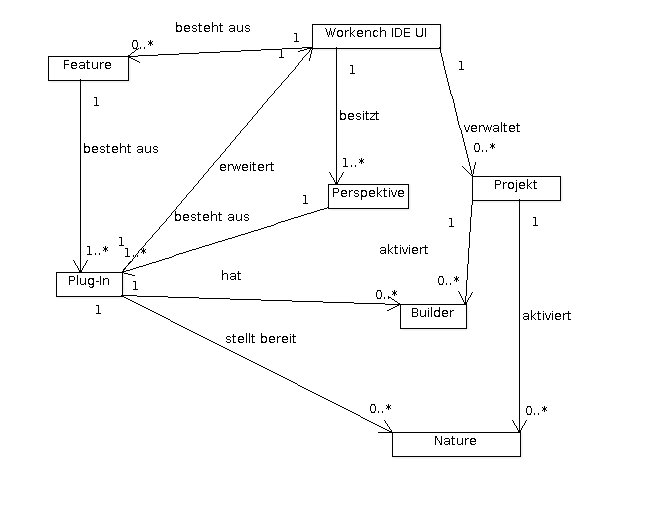
\includegraphics[width=500px]{diagramme/eclipse-beziehung.png}
		\caption{Beziehungen zwischen den einzelnen Eclipse-Komponenten}
		\label{fig:eclipse-beziehungen}
\end{figure}

\section{Eclipse Modeling Framework}
Das Eclipse Modeling Framework besteht aus verschiedenen Plug-ins für die Eclipse-Plattform um eigene  Metamodelle abbilden zu können. Die Erstellung dieser  Metamodelle geschieht dabei über grafische Tools, die wiederum das  Metamodell innerhalb eines eigenen XML-Dialekts konvertieren. Diese XML-Dateien werden mit der Endung \textit{.ecore} gespeichert.
EMF stellt weiterhin einen Generator bereit, der aus der Ecore-Datei Java-Klassen erzeugt. Diese werden von der Applikation als Grundlage für die Domänenobjekte genutzt. 
\section{ANTLR}
Um  Metamodelle mit Hilfe einer eigenen domänenspezifische Sprache zu definieren, sind in aller Regel zwei Komponenten nötig: Der \textit{Lexer} kümmert sich um das Zerlegen des Eingabestreams in logisch zusammenhängende Zeichenfolgen, die sogenannten Token\footnote{Scannerless Parser wie zum Beispiel zum Parsen von TeX sind Ausnahmen von der Regel und benötigen keinen eigenen Lexer}. Die Token werden anschließend vom \textit{Parser} als Grundlage für weitere Operationen genommen. Dazu zählt unter anderem die Überprüfung, ob die zugrundeliegende Grammatik syntaktisch gültig ist. Die Grammatik legt dabei die Regeln fest, in welcher Weise die Sprachelemente der DSL genutzt werden müssen.
Für das automatische Erstellen von Lexern und Parsern existieren einige Tools wie z.B. yacc, JavaCC oder ANTLR. Xtext nutzt intern zum Parsen der DSLs bzw. Grammatiken das Tool ANTLR (\textit{Another Tool for Language Recognition}).
\section{Xtext}
Für die vorliegende Arbeit wurde Xtext als Tool für externe DSLs ausgewählt. Xtext nutzt die Eclipse IDE als Grundlage für die Generierung. Unter anderem spielten bei der Entscheidung folgende Aspekte eine Rolle:
\begin{itemize}
	\item Die Entwicklung von Xtext wird von der itemis AG getrieben. Die Mitarbeiter entwickeln aktiv an der Software und präsentieren ihre Ergebnisse in Java User Groups, in Blogs und bei großen Java-Konferenzen. Probleme werden per Twitter oder über das offizielle Xtext-Forum\footnote{http://www.eclipse.org/forums/index.php?t=thread\&frm\_id=27} von den Entwicklern sehr schnell beantwortet.
	\item Die Einstiegshürde in Xtext fällt durch die sehr gute Dokumentation und vorhandene Beispiele sehr einfach aus.
	\item Xtext erzeugt für die DSL eigene Plug-ins für Eclipse. Funktionalitäten wie Autovervollständung und Syntax Highlighting innerhalb des Editors der DSL sind somit automatisch vorhanden. Die Erweiterung um eigene Funktionalitäten ist verhältnismäßig einfach.
	\item Xtext ist Open Source. Bei Problemen oder Verständisschwierigkeiten von Xtext kann man mit einem Debugger die internen Abläufe innerhalb der Eclipse-Umgebung nachverfolgen.
\end{itemize} 

Xtext selbst besteht aus mehreren Plug-ins für Eclipse. Eigene DSLs werden über die Xtext-Grammatik definiert. 
Über das Java-Tool ANTLR werden für die DLSs Lexer und Parser generiert, die entstehenden Java-Klassen werden hingegen von Xtext/XPand erzeugt. 
Die Xtext-Grammatik ist dabei selbst in Xtext definiert \cite{xtextXtext}. Xtext kann sich somit selbst erzeugen.
\\
Xtext erzeugt aus den geschriebenen Grammatiken automatisch das Grundgerüst für eigene Eclipse Plug-ins. Weiterhin wird durch die integrierten Plug-ins des Eclipse Modeling Frameworks ein vollständiges Ecore-Metamodell der DSL generiert.
Mit Hilfe von Lexer und Parser wird das Modell der DSL geparst und in ein Objektbaum auf Basis von Ecore transformiert. Über diesen Abstract Syntax Tree kann Java auf die Inhalte der DSL zugreifen.\\
Jedes Element innerhalb des Objektbaums beinhaltet die Referenzen zu Eltern- und Kindelementen. Somit kann von jedem Element aus über das komplette Metamodell iteriert werden.
\subsection{Xbase}
Xbase ist eine statisch-typisierte Programmiersprache, die selbst in einer Xtext-Grammatik definiert worden ist \cite{xbaseXtext}.
Sie stellt unter anderem Lambda-Ausdrücke bereit und kann Operatoren überladen \cite{xbaseIntro}. Über Type Inferencing kann auf die volle Klassenhierarchie von Java zugegriffen werden.\\
In einer eigenen DSL kann Xbase eingesetzt werden, um diese um Ausdrücke zu erweitern. Eigene Programmlogik kann so innerhalb der DSL untergebracht werden \textbf{ohne} dass eigene Grammatiken definiert werden müssen.
Xbase wird unter anderem von den Xtext-Komponenten Xtend und MWE benutzt.
\subsection{Xtend}
Die Xtext-Entwicklungsumgebung stellt die statisch-typisierte Pro\-gram\-mier\-spra\-che Xtend bereit. Xtend unterstützt unter anderem Lambda-Expression und Extension Methods. Xtend ist durch eine Xtext-Grammatik definiert Quellen liegen unter \cite{xtendXtext} und nutzt Xbase.\\
Der Builder von Xtend erzeugt Java-Quellcode, der wiederum durch durch den Compiler zu lauffähigem JVM-Bytecode umgewandelt wird.
Xtend soll als leichtgewichtige Programmiersprache und Alternative zu Java dienen. Die Programmiersprache ist fest in das Xtext-Framework integriert: neben den Stan\-dard\-funk\-tionalitäten, die Xtext für generierte DSLs bereitstellt, existiert ebenfalls Debugging Support in Eclipse.\\
Durch die Unterstüzung von Template Expressions \cite{xtendDoc} innerhalb von Textblöcken eignet sich diese Programmiersprache besonders für die Transformation der eigenen DSL in ein Ausgabeartefakt: Der Entwickler kann z.B. innerhalb eines Textsegments über ein Array iterieren:
\begin{verbatim}
var personen = ["Trinity", "Neo", "Morpheus"] 
var artefakt = '''
  <ul>
  «FOREACH person : personen»
    <li>«person»</li>
  «ENDFOREACH»
  </ul>
'''
\end{verbatim}
Strings werden durch drei Hochkommata ein\-ge\-schlossen. Innerhalb dieses Blocks können XPand-Ausdrücke in Guillemot-Pfeilen genutzt werden. XPand-Ausdrücke haben dabei Zugriff auf die definierten Variablen innerhalb des Objekts oder der Methode. Eclipse unterstützt innerhalb dieser Ausdrücke Autovervollstän\-di\-gung.\\
Im Beispiel würde über das Array \verb-personen- iteriert und der entstehende String in der Variablen \verb-artefakt- gespeichert werden. Der entstehende String würde dann wie folgt aussehen:
\begin{verbatim}
  <ul>
    <li>Trinity</li>
    <li>Neo</li>
    <li>Morpheus</li>
  </ul>
\end{verbatim}
\subsection{MWE}
Um wiederkehrende Arbeitsabläufe wie z.B. die Generierung von Code zu automatisieren, wird innerhalb der Xtext-Plattform die Modeling Workflow Engine genutzt.
Die Modeling Workflow Engine besitzt eine eigene DSL, mit der beschrieben wird, in welcher Reihenfolge einzelne Arbeitsabläufe ausgeführt werden müssen.
Die Grammatik der MWE-DSL ist dabei in einer Xtext-Grammatik definiert, die Xbase unterstützt\footnote{http://www.eclipse.org/modeling/emft/downloads/?project=mwe, SDK MWE2 (Runtime, Source), /eclipse/plugins/org.eclipse.emf.mwe2.language.source\_2.3.0.v201206120758.jar, /org/eclipse/emf/mwe2/language/Mwe2.xtext}. Eigene Komponenten können durch die Implementierung des Java-Interfaces \textit{IWorkflowComponent} bereitgestellt werden.
\\
\\
Xtext generiert beim Erstellen einer neuen DSL automatisch eine Workflow-Definition, die dann für die weitere Code-Generierung der DSL-Infrastruktur genutzt wird.
Anhand des folgenden Quellcode-Fragments soll kurz die Grammatik und Funktionsweise von MWE beschrieben werden:
\begin{verbatim}
var projectName = "de.ckl.rapid"
var runtimeProject = "../${projectName}"
Workflow {
    // ... weitere Instruktionen
    component = DirectoryCleaner {
        directory = "${runtimeProject}/src-gen"
    }
    // ... weitere Instruktionen
}
\end{verbatim}

Mit dem Schlüsselwort \texttt{var} werden Variablen definiert, die später wiederverwendet werden können. Auf Variablen können innerhalb von Zeichenketten mit Hilfe des Konstrukts \texttt{\$\{...\}} referenziert werden.
Mit Hilfe des Wortes \texttt{Workflow} wird eine neue Instanz der Klasse \texttt{Workflow}\footnote{org.eclipse.emf.mwe2.runtime.workflow.Workflow} erzeugt. Hier können auch beliebig andere Klassen genutzt werden, die das Interface \texttt{IWorkflow} implementieren.
\\
\\
Innerhalb des \texttt{Workflow}-Blocks, gekennzeichnet durch die geschweiften Klammern, können nun Komponenten mit Hilfe des Schlüsselwortes \texttt{component} definiert werden. Diese werden der Reihe nach ausgeführt. Im obigen Beispiel wird eine neue Komponente eingefügt, indem eine neue Instanz der Klasse\\
 \texttt{DirectoryCleaner}\footnote{org.eclipse.emf.mwe.utils.DirectoryCleaner} instanziert wird. In der Instanz wird die Bean-Eigenschaft \texttt{directory} zugewiesen.
Komponenten müssen das Interface \texttt{IWorkflowComponent}
\footnote{org.eclipse.emf.mwe2.runtime.workflow.IWorkflowComponent} implementieren. Beim Setzen der Eigenschaft \texttt{directory} wird durch MWE automatisch die Setter-Methode \texttt{setDirectory(...)} aufgerufen.
\\
\\
Wie man an dem Codefragment erkennen kann, ist MWE ein gutes Beispiel für eine domänenspezifische Sprache, da sich die Grammatik allein auf die relativ einfache Problemdomäne \textit{Sequenzielles Ausführen von Workflows} konzentriert.
\subsection{Guice}
Das komplette Xtext-Framework nutzt das Dependency Injection-Framework Guice, das von Google entwickelt und als Open Source-Software veröffentlicht wurde.
Im Gegensatz zum DI-Framework Spring ist Guice leichtgewichtiger\footnote{guice-3.0.jar, aopalliance.jar javax.inject.jar sind kleiner als 720 KByte}.
Klassen, die das Interface \verb+Module+ implementieren, definieren die Bindings von Schnittstellen zu Klassen. Eine Konfiguration der Abhängigkeiten über XML-Dateien wie es in Spring möglich ist, ist standardmäßig nicht vorhanden.\\
Durch das Überschreiben von bestehenden Bindings können innerhalb des Xtext-Plug-ins eigene Klassen injiziert werden.\\
Neue Objektinstanzen werden nun über Guice erzeugt. Alle Abhängigkeiten werden anhand der in der Moduldefinition gebundenen Interfaces injiziert.
Xtext generiert Moduldefinitionen mit dem Suffix \emph{Module}. Innerhalb der Klasse \verb+RapidUiModule+ wird z.B. mit Hilfe der folgenden Methode das Interface \verb+IXtextBuilderParticipant+ an die konkrete Implementierung \verb+MultipleBinderParticipant+ gebunden:
\begin{verbatim}
public Class<? extends org.eclipse.xtext.builder
    .IXtextBuilderParticipant>
    bindIXtextBuilderParticipant() {
    return de.ckl.rapid.ui.builder.MultipleBuilderParticipant.class;
}
\end{verbatim}
In jeder Klasse, die von Guice erstellt wird, bekommen nun alle Attribute mit der Annotation \emph{@Inject} die zugehörige gebundene Instanz injiziert:
\begin{verbatim}
    @Inject
    IXtextBuilderParticipant builderParticipant;
\end{verbatim}
\subsection{Erstellung einer neuen DSL}
\newcommand{\paketname}[0]{{\textit{\${paket.name}}}}
\newcommand{\dslname}[0]{{\textit{\${dsl-name}}}}
\begin{itemize}
	\item Der Benutzer erstellt innerhalb der Eclipse-Umgebung ein neues Xtext-DSL-Projekt.
	Dabei muss er den Namen der DSL \dslname, sowie den Paketnamen der DSL \paketname\ definieren.
	\item Das Eclipse Plug-in des Xtext-Frameworks generiert daraufhin automatisch drei Eclipse Plug-ins:
	\begin{itemize}
		\item \paketname: Grundgerüst für das DSL-Backend. Dieses enthält den Parser, Lexer, Formatter,  Metamodell, Scoping- und Validation-Provider. Der generierte Quellcode ist standardmäßig nicht abhängig von der Eclipse-Laufzeitumgebung und kann auch in Konsolen- oder Webanwendungen wiederverwendet werden.
		\item \paketname.test: Grundgerüst für das Ausführen von Unittests
		\item \paketname.ui: Grundgerüst für das User Interface. Dies beinhaltet unter anderem Content Assistents, Quickfixing und Outline Views. Der generierte Quellcode hängt dabei direkt von Eclipse IDE ab und kann ohne diese nicht ausgeführt werden.
	\end{itemize}
	Jegliches Customizing durch den Benutzer darf nur innerhalb der \textit{src}-Ver\-zeich\-nisse in den Projektordnern geschehen. Alle Änderungen im Ordner \textit{src-gen} werden beim Neuerstellen des Backends (z.B. bei Änderungen der Grammatik) überschrieben.
	\item Der Benutzer definiert innerhalb des Projekts \${paketname}:/src/\paketname/\dslname.xtext die Grammatik der DSL
	\item Der Benutzer startet über den Menüpunkt \textit{MWE2 Generate artifact} den Workflow zum Generieren des Backends
	\item Der MWE2-Workflow erzeugt nun im Verzeichnis \paketname:/src-gen das komplette Backend. Ecore-Metamodell, Parser und Lexer werden neu ge\-ne\-riert.
	\item Der Benutzer implementiert nun eigene Funktionalitäten, indem er seine eigenen Implementierungen in einer der Moduldateien bindet.
\end{itemize}
\chapter{Realisierung}
\label{ch:realisierung}
Nachdem die grundlegenden Technologien erklärt worden sind, folgt nun die Beschreibung der Realisierung.
Als erstes wurde das in der Grafik \ref{beispiel-applikation} sichtbare UML-Diagramm einer Beispielapplikation erstellt, deren Anforderungen durch die DSL abgedeckt werden sollten. Der Einfachheit halber beschränkte es sich auf eine Forumsanwendung. Dabei wurden neben einfachen 1:n-Beziehungen auch die Möglichkeit gegeben, dass Benutzer in der Rolle \textit{Moderator} über eine assoziative Klasse beliebig viele Foren moderieren können.
Weiterhin besitzt die Klasse \textit{Post} eine reflexive Assoziation, so dass eine Baumstruktur der Postings abgebildet werden kann.
Die Methoden sind der Übersichtlichkeit halber ausgeblendet.

\begin{figure}[h]
	\centering
		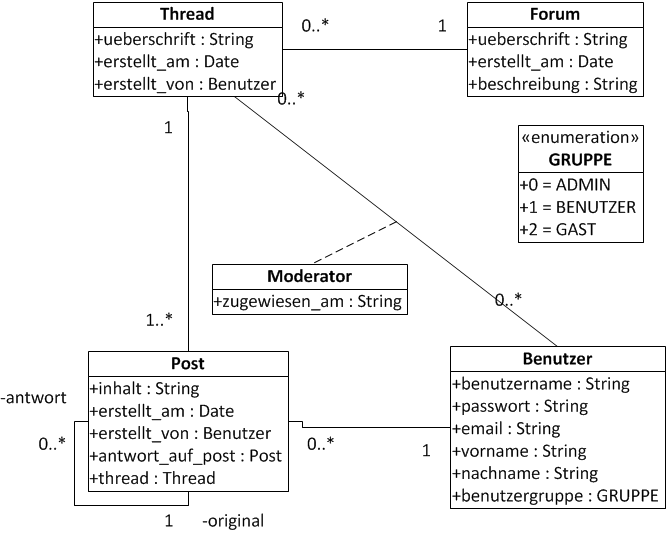
\includegraphics[width=400px]{diagramme/beispiel-applikation.png}
		\caption{Beispielapplikation eines Forums}
		\label{fig:beispiel-applikation}
\end{figure}

\section{Definition und Umsetzung des  Metamodells}
Nach dem Design des UML-Diagramms wurde auf dieser Grundlage ein Prototyp des  Metamodells erstellt. 

Die Erstellung des Prototypen orientierte sich dabei an den Fragen:
\begin{itemize}
	\item \textit{Lässt sich die Sprache für einen Softwareentwickler intuitiv benutzen?} Bekannte Sprachkonstrukte aus verbreiteten Programmiersprachen sollten wiederverwendet werden.
	\item \textit{Sind die Schlüsselwörter meiner Sprache eingängig?} Die Schlüsselwörter der Sprache müssen einerseits aussagekräftig sein, andererseits aber auch ein gewisses Maß an Abstraktion besitzen.
	\item \textit{Kann ich mit dieser Sprache meine Beispielanwendung abbilden?} Die Sprache muss in der Lage sein, Kardinalitäten, Attribute, Klassen und Assoziationen abzubilden.
	\item \textit{Ist der Detaillierungsgrad meiner Sprache zu hoch?} Das Entwerfen einer Sprache von Grund auf hat den Nachteil, dass man sich sehr schnell in Details verlieren kann.
	Angenommen, es gilt die Konvention, dass Datums\-werte immer als Zeitstempel gespeichert werden, dann ist es nicht nötig, dass ein Datentyp \textit{date} neben dem Datentyp \textit{datetime} eingeführt wird.
\end{itemize}
Der Prototyp wurde iterativ entwickelt, bis letztendlich eine Grammatik gefunden wurde, bei der alle Fragen zufriedenstellend beantwortet werden konnten. Als Projektname für die DSL wurde \textit{Rapid} mit dem in Grafik \ref{rapid-log} zu sehenden Logo gewählt. Die  Grammatik und Sprachelemente dieser DSL wird in den folgenden Unterkapiteln beschrieben.
\begin{figure}[h]
	\centering
		
\includegraphics[width=350px]{img/rapid-logo.png}
		\caption{Das Logo von Rapid}
		\label{fig:rapid-logo}
\end{figure}

\subsection{Allgemeiner Aufbau}
Ein Modell wird in aller Regel innerhalb einer Datei definiert. Xtext erlaubt es allerdings, dass das Modell auch in mehreren Dateien zur Verfügung steht. So lassen sich bestimmte Komponenten auslagern. 
\begin{itemize}
	\item Kommentare innerhalb des Modells oder Metamodells werden standardmäßig über \verb+//+ oder \verb+/* ... */+ definiert.
	\item Wenn mehrere Elemente zusammengefasst werden sollen, wird dies durch eckige Klammern dargestellt. Hier wurde die Deklarierung von Arrays aus Programmiersprachen wie C oder Java übernommen.
	\item Innerhalb von Domänen kann das Schlüsselwort \textit{self} benutzt werden, um auf die Domäne zu verweisen, in der sich das Element befindet.
	\item Zur Definition von Kardinalitäten im Metamodell werden die Token \textit{*} (0..n), \textit{?} (0..1) und \textit{+} (1..n) genutzt. Wurde keine Kardinalität angegeben, gilt immer, dass das Element genau einmal vorkommen muss. Die weitere Syntax kann unter \cite{xtextDocumentation} eingesehen werden.
\end{itemize}
Das Metamodell zum allgemeinen Aufbau sind folgendermaßen aus:
\begin{verbatim}
Model:
    (imports+=Import)*
    (('application' '{'
        ('name:' applicationName=STRING) &
        ('package:' package=QualifiedName)
        ('navigation:' ...
        )?
    '}'
    )?
    (enums+=Enum)*
    (types+=Type)*
    (domains+=Domain)* 
    )
;

Import:
	'import' importedNamespace=QualifiedNameWithWildcard
;

QualifiedNameWithWildcard:
  QualifiedName '.*'?
;
\end{verbatim}
Jedes Modell kann beliebige JVM-Klassen über das Schlüsselwort \textit{import} importieren. Diese Funktionalität ist nötig, wenn man Annotationen wie in Kapitel \ref{sec:annotationen} benutzen und nicht immer den vollqualifizierten Namen der Annotation schreiben will.
Eine Applikation muss einen Namen (\textit{name}) beinhalten und einen Namensraum definieren (\textit{package}).
Nach dieser Präambel folgt die optionale Deklaration von Enumerationen, Typen und Domänen.
Für die Beispielanwendung könnte folgendes Modell genutzt werden:
\begin{verbatim}
// Annotation importieren
import de.ckl.rapid.artifact.fpanalysis./*...*/.UseFunctionpointType

application {
    name: "Forumsanwendung"
    package: de.ckl.apps.forum
}

// Enumerationen
// Typen
// Domänen
\end{verbatim}

\subsection{Enumerationen}
\label{sub:enumerationen}
Eine Enumeration ist ein Datentyp zur Aufzählung von Werten. Rapid stellt Enumerationen bereit und orientiert sich dabei an der Nutzung von Aufzählungen, wie sie in C\# verwendet werden:
\begin{verbatim}
Enum:
    'enum' name=ID '[' 
        values+=EnumValue (',' values += EnumValue)* 
    ']'
;

EnumValue:
    name=ID ('=' value=INT)?
;

EnumDataType:
    'enum' '(' refEnum=[Enum] ')'(nullable?='?')?
;
\end{verbatim}
Eine Enumeration wird dem Schlüsselwort \textit{enum} definiert. Soll später auf diese Aufzählung verwiesen werden, muss ebenfalls \textit{enum} benutzt werden. Danach folgt der Name der zu nutzenden Enumeration innerhalb der Klammern. Mit dem Fragezeichen \textit{?} kann gekennzeichnet werden, dass die Nutzung dieses Datentyps NULL-Werte erlaubt.
Innerhalb der Forumsapplikation können Enums zur Definition von Benutzergruppen genutzt werden:
\begin{verbatim}
// Definition der Enumeration
enum GRUPPE [0 = ADMIN, 1 = BENUTZER, 2 = GAST]

domain Benutzer {
    // Referenz zur Enumeration GRUPPE; Attribut kann null sein
    attr benutzergruppe: enum(GRUPPE)?
}
\end{verbatim}
\subsection{Datentypen}
Rapid enthält eine Grundmenge an Datentypen wie \textit{string}, \textit{long}, \textit{double}, \textit{boolean} und \textit{datetime}. Diese können je nach Gültigkeitsbereich NULL sein. Allerdings reichen in aller Regel diese Datentypen nicht aus und oft kommt es vor, dass man bestehende Datentypen verwenden oder neue Datentypen einführen will.
Um diese Anforderung umzusetzen, wurde das Schlüsselwort \textit{type} definiert und die Annotation \textit{@MapToBackend} implementiert. Die formale Definition erlaubt, dass jeder neu definierte Datentyp annotiert werden kann:
\begin{verbatim}
Type:
    (annotations+=XAnnotation)*
    'type' name=ID
;

CustomDataType:
    'type' '(' refType=[Type] ')'(nullable?='?')?
;
\end{verbatim}
Innerhalb des Modells kann nun z.B. dem Benutzer ein Attribut namens \textit{guid} zuordnen, dass auf den Datentyp \textit{System.Guid} aus dem .NET-Framework gemappt wird. Die Auswertung des Mappings muss dabei natürlich immer von den Generatoren erfolgen.
\begin{verbatim}
@MapToBackend("System.Guid")
type Guid

domain Benutzer {
    attr guidInActiveDirectory: type(Guid)?
}
\end{verbatim}

\subsection{Domänen}
Domänen beschreiben letztendlich die Klassen einer Applikation:
\begin{verbatim}
Domain:
(annotations+=XAnnotation)*
'domain' name=ID 
('extends' refParentDomain=[Domain] 
    ('as' parentDomainLabel=STRING)?)? 
    '{'
    ('label:' label=STRING)?
    ('description:' description=STRING)? 
    (attributes+=Attribute)*
    (fieldgroups+=Fieldgroup)*
    (references+=HasManyReference)*
    (processes+=Process)*
    ('options' '{'
    (
        ('examples:' '[' 
            examples+= STRING (',' examples+=STRING)* 
        ']')?
    )
    '}')?
'}'
;
\end{verbatim}
Domänen können mit Annotationen ausgestattet werden und von anderen Domänen erben (\textit{extends}). Die Vererbung ist optional. Zirkuläre Referenzen sind durch einen passenden Validator nicht möglich.
Jede Domäne kann ein Label (\textit{label}) und Beschreibung (\textit{description}) besitzen. Innerhalb einer Domäne können beliebig viele Attribute, Referenzen, Prozesse und Feldgruppen definiert werden. Feldgruppen fassen mehrere Attribute zu einer Gruppe zusammen und ermöglichen beispielsweise in einer Oberfläche die Gruppierung von Eingabeelementen. Attribute sind entweder Felder von einfachen Datentypen oder Referenzen auf eigene Datentypen, Enumerationen oder andere Domänen. Eine Referenz auf eine andere Domäne kann als ``gehört zu`` oder ``hat eine`` gelesen werden. Many-To-Many-Referenzen werden in Kapitel \ref{sec:multiplizitaeten} näher beschrieben. 

Mit all diesen Elementen lässt sich eine Thread-Domäne der Beispielapplikation implementieren:
\begin{verbatim}
domain Thread {
    attr ueberschrift: string
    attr erstellt_am: datetime
    erstellt_von: Benutzer
    has-many posts: Post(mapped-by Post.thread)
}
\end{verbatim}
\subsection{Prozesse}
Prozesse bilden innerhalb der Domäne User Stories ab, die während des Requirements Engineering aufgenommen worden sind:
\begin{verbatim}
Process:
    (annotations+=XAnnotation)*
    'process' name=ID ('{'
        ('label:' label=STRING)?
        ('description:' description=STRING)? 
        ('view:' view=('detail' | 'edit' | 'list' | 'statistic')
            ('[' 
                referencesForView+=AttributeReference 
                (',' referencesForView+=AttributeReference)*
             ']'
            )?
        )?
        ('delegates-to:' '[' 
            delegatesTo+=Transition (',' delegatesTo+=Transition)* 
        ']')?
    '}')?
;
\end{verbatim}
Neben den bereits bekannten Annotationen und Schlüsselwörtern \textit{label} und \textit{description} existieren innerhalb des Prozess-Kontextes die Schlüsselwörter \textit{view} und \textit{delegates-to}. Mit \textit{view} wird definiert, welche Ausgabe dieser Prozess erzeugt, sobald er gestartet worden ist. Es folgen in eckigen Klammern alle Attribute, die innerhalb der Ausgabe angezeigt werden sollen. Über \textit{delegates-to} wird gesteuert, an welche weiteren Prozesse dieser Prozess delegieren kann.
Damit ließe sich beispielsweise eine Eingabemaske für neue Benutzer definieren, die nach Fertigstellung an den Prozess \verb+listBenutzer+ weiterleitet:
\begin{verbatim}
domain Benutzer {
    // Attribute
    process addBenutzer {
        label: "Neuen Benutzer hinzufügen"
        description: "Fügt einen neuen Benutzer hinzu"
        view: edit [
            self.passwort,
            self.email,
            self.vorname, 
            self.nachname
        ]
        delegates-to: [ listBenutzer ]
    }

    process listBenutzer {
        label: "Alle Benutzer anzeigen"
        view: list
    }
}
\end{verbatim}
\subsection{Referenzen}
Referenzen sind Verweise auf Attribute, Prozesse oder Multiplizitäten innerhalb der selben oder einer anderen Domäne. Ursprünglich sollte dabei folgende Grammatik genutzt werden:
\begin{verbatim}
	Domaene->Attribut
	bzw. Domaene->Prozess
	bzw. Domaene->Multiplizitaet
\end{verbatim}
Die Eindeutigkeit der Namen von \textit{Attribut}, \textit{Multiplizitaet} und \textit{Prozess} hätten dabei über Validatoren sichergestellt werden sollen. Aller\-dings kann ANTLR nicht unterscheiden, welches Element nach dem Schlüsselwort ``\verb+->+`` genommen werden soll. Die Problematik konnte ebenfalls nicht mit Syntactic Predicates gelöst werden. Stattdessen werden die unterschiedlichen Typen von Referenzen über das Token zwischen der Domäne und dem Namen der Referenz unterschieden:
\begin{verbatim}
	Domaene.Attribut
	bzw. Domaene->Prozess
	bzw. Domaene*Multiplizitaet
\end{verbatim}
\subsection{Multiplizitäten}
\label{sec:multiplizitaeten}
Ein wichtiger Teil einer jeden DSL besteht darin, Multiplizitäten zwischen einzelnen oder mehreren Domänen zu definieren. In Rapid existieren vier Möglichkeiten um Multiplizitäten zu definieren. Bei der Nutzung des Schlüsselwortes \textit{has-many} bzw. \textit{belongs-to} ist es immer nötig, dass der Endpunkt in der referenzierten Domäne benannt wird. Dies kann entweder ein Attribut oder eine Multiplizität sein. Dieses Vorgehen ist nötig, um eine eindeutige Zuordnung zwischen Domänen zu erstellen. Als Vorbild diente das Mapping-Konzept der Java Persistence API \cite{javaapi5ManyToMany}, \cite{javaapi5ManyToOne}.
Die Unterscheidung zwischen \textit{has-many} und \textit{belongs-to} wird von der DSL nicht aktiv berücksichtigt, sondern dient alleine dem Anwender zur intuitiven Bedienung der DSL.

Bei folgendem Code wird definiert, dass die Domäne \verb+D1+ der Domäne \verb+D2+ angehört. Der Domäne \verb+D2+ ist diese Verbindung nicht explizit bekannt. Es besteht eine 1:n-Beziehung zwischen D2:D1.
\begin{verbatim}
domain D1 {
    attr d2: D2
}

domain D2 {
}
\end{verbatim}

Um nun der Domäne \verb+D2+ die Verbindung bekannt zu machen, wird das \textit{has-many}-Attribut genutzt. Dieses Konstrukt verlangt, dass in der referenzierten Domäne der Endpunkt benannt wird:
\begin{verbatim}
domain D1 {
    attr d2: D2
}

domain D2 {
    has-many d1: D1(mapped-by D1.d2)
}
\end{verbatim}

Soll eine m:n-Beziehung hergestellt werden, müssen beide Domänen mit \textit{has-many}-Schlüsselwörtern ausgestattet werden. Referenzen werden mit Hilfe des Sternchens \verb+*+ von Attributen unterschieden:
\begin{verbatim}
domain D1 {
    has-many d2: D2(mapped-by D2*d1)
}

domain D2 {
    has-many d1: D1(mapped-by D1*d2)
}
\end{verbatim}

Die letzte Möglichkeit besteht darin, dass eine m:n-Beziehung mit Hilfe einer Assoziationsdomäne hergestellt wird. Im letzten Beispiel stellt die Domäne \verb+A1+ die Verbindung zwischen den beiden Domänen her:
\begin{verbatim}
domain D1 {
    has-many d2: D2(mapped-by A1.d1)
}

domain D2 {
    has-many d1: D1(mapped-by A1.d2)
}

domain A1 {
    attr d1: D1
    attr d2: D2
}
\end{verbatim}

Innerhalb der DSL wird durch passende Quickfixes und Validatoren der korrekte Einsatz der Multiplizitäten sichergestellt.
\section{Erweiterung der Ba\-sis\-funk\-tio\-na\-li\-tä\-ten von Xtext}
Werden die Xtext-Artefakte generiert, erzeugt Xtext anhand der DSL alle Klassen, die für das eigene Eclipse Plug-in nötig sind. Dieser Vorgang muss mit jeder Änderung an der DSL manuell ausgeführt werden.
Bei der ersten Generierung werden alle Dateien innerhalb der Ordner \emph{src-gen} erzeugt. Diese dürfen vom Entwickler nicht angepasst werden, da bei jeder Änderung an der Grammatik eine neue Neuerstellung dieser Dateien stattfindet.
Die eigentliche Implementierung geschieht in den .java-Dateien des Ordners \emph{src}. Xtext nutzt als Präfix für die Klassen den Namen der DSL, so dass jede automatisch generierte Klasse innerhalb der \emph{src}-Ordner mit \verb+Rapid+ beginnt. Diese Klassen werden einmalig beim ersten Lauf der Artefakt-Generierung erzeugt und werden nicht überschrieben.
\\
\\
Die Architektur der gesamten Xtext-Infrastruktur erlaubt es auf einfache Art und Weise der DSL Features hinzuzufügen, die den Anwender beim Umgang mit der Sprache unterstützen.
Im Folgenden soll ein kurzer Einblick gegeben werden, welche Features angepasst worden sind.
\label{subsec:scoping}
\subsection{Scoping}
Scoping bedeutet, dass innerhalb eines bestimmten Kontextes nur die Teilmenge eines bestimmten Typs erlaubt ist. Die Auswahl der erlaubten Elemente wird also eingeschränkt.
\\Xtext generiert standardmäßig die Klasse \verb+RapidScopeProvider+, in der das Scoping definiert werden kann. Die Nutzung von Annotationen\footnote{siehe Kaptiel \ref{sec:annotationen}}  macht es nötig, dass zwei verschiedene Scope Provider implementiert werden:
\begin{itemize}
	\item Die Klasse \verb+RapidScopeProvider+ erbt von \verb+XbaseWithAnnotationsScopeProvider+\footnote{org.eclipse.xtext.xbase.annotations.scoping.XbaseWithAnnotationsScopeProvider}. Darüber wird sichergestellt, dass Annotationen per Autovervollständigung innerhalb des Editors angezeigt werden können. Das Scoping wird an die Klasse \verb+RapidDeclarativeScopeProvider+ delegiert.
	\item Innerhalb von \verb+RapidDeclarativeScopeProvider+ können eigene Scopings implementiert werden, indem eine neue Methode mit der benötigten Signatur \verb+scope_$Rückgabeelement($KontextElement, EReference)+ erstellt wird. Der folgende Quellcode liefert alle erlaubten Attribute zurück, die innerhalb des Elements \verb+Fieldgroup+ verfügbar sind:
	\begin{verbatim}
	IScope scope_Attribute(Fieldgroup ctx, EReference ref) {
	    return scopeFor(((Domain)ctx.eContainer()).getAttributes())
	}
	\end{verbatim}
\end{itemize}


In Rapid wurden Scopings definiert, um die Auswahl von Prozessen, Attributen und Referenzen einzuschränken. 
Folgender Auszug aus Rapid stellt eine 1-n Beziehung zwischen der Domäne \verb+MyDomain+ und \verb+OtherDomain+ her:
\begin{verbatim}
domain MyDomain {
    has-many od: OtherDomain(mapped-by: OtherDomain.belongsToMyDomain)
}

domain OtherDomain {
    attr belongsToMyDomain: MyDomain
    attr otherAttribute: string
}
\end{verbatim}

Ohne Scoping würden bei der Autovervollständigung hinter \verb+mapped-by: OtherDomain+ die beiden Attribute \verb+belongsToMyDomain+ und \verb+otherAttribute+ vorgeschlagen werden.
Da das Gegenstück einer Referenz immer vom selben Typ sein muss, in dem sich der Cursor gerade befindet, ist das Attribut \verb+otherAttribute+ nicht erlaubt. Das Scoping filtert im Beispiel alle Elemente heraus, die nicht vom Typ \verb+MyDomain+ sind und in der Autovervollständigung erscheint deshalb nur \verb+belongsToDomain+.
Sollte der Anwender manuell eine andere Referenz eintragen, wird dies als semantischer Fehler markiert. Dieser muss vom Anwender behoben werden, da sonst der Buildprozess nicht gestartet werden kann.
\subsection{Validation}
Um einzelne Elemente auf ihre Gültigkeit zu überprüfen, erzeugt Xtext die Klasse \verb+RapidJavaValidator+. Jede dort mit \textit{@Check} annotierte Methode wird aufgerufen, sobald eine Ausprägung der DSL gespeichert wird.
Mit Hilfe der Methoden \verb+error()+, \verb+warning()+ und \verb+info()+ können zu validierende Elemente mit einer eindeutigen Validator-ID markiert werden. Diese werden dann in der \emph{Problem View} von Eclipse aufgelistet.

Im konkreten Fall wurden unter anderem Validatoren implementiert, um
\begin{itemize}
	\item zu erzwingen, dass nur Annotationen benutzt werden dürfen, die selbst mit \verb+@Attribute+, \verb+@Process+, \verb+@Domain+, \verb+@HasManyReference+ oder \verb+@Type+ annotiert sind.
	\item zu verhindern, dass zirkuläre Abhängigkeiten zwischen vererbten Domänen entstehen.
	\item das Benutzen des Attribut-Namens \textit{id} zu verbieten, da dieses Attribut für jede Domäne automatisch gesetzt wird.
	\item doppelte Attribute-, Prozess- oder Referenznamen innerhalb von Domänen zu unterbinden.
	\item das doppelte Vorhandensein von Enumeration-Werten zu verhindern.
	\item die korrekte Benutzung von m:n-Beziehungen zu überprüfen.
	\item doppelte Nutzung von Attributen innerhalb von Feldgruppen zu verhindern
\end{itemize}

Einen Sonderfall nehmen die Validatoren mit dem Präfix \verb+provide+ ein. Diese markieren bestimmte Stellen innerhalb der DSL als ``informativ``, so dass mit Hilfe von Quickfixes alternative Lösungswege beschritten werden können.
\begin{itemize}
	\item \verb+provideAddCrudOperationQuickfix(...)+ sorgt dafür, dass wenn eine Do\-mä\-ne keinen Prozess mit dem Namen \verb+create+, \verb+delete+ oder \verb+update+ besitzt, dieses per Quickfix automatisch erstellt werden kann.
	\item \verb+provideIntroduceOfAssociationTable(...)+ markiert die betreffende Stelle, wenn zwischen zwei Domänen eine direkte m:n-Beziehung existiert, ohne dass eine explizite Assoziationsdomäne hinzugefügt worden ist.
\end{itemize}

Der folgende Code überprüft beispielsweise, ob der Attributname in einer Domäne doppelt vorhanden ist:
\begin{verbatim}
@Check
public void noDuplicateAttributeNameInDomain(Attribute attribute) {
    Domain self = (Domain) attribute.eContainer();
    List<String> names = new ArrayList<String>();

    for (Attribute a : self.getAttributes()) {
        if (names.contains(a.getName())) {
            error("Das Attribut mit dem Namen \"" + a.getName()
                + "\" ist in der Domäne \"" + self.getName()
                + "\" bereits definiert worden.", attribute,
                RapidPackage.Literals.ATTRIBUTE__NAME,
                ERROR_ATTRIBUTE_NAME_ALREADY_EXISTS);
        }
        
        names.add(a.getName());
    }
}
\end{verbatim}

\subsection{Formatting}
Xtext stellt über die Klasse \verb+RapidFormatter+ die Möglichkeit bereit, dass eine Ausprägung einer DSL über die Tastaturkürzel \textit{Strg+Shift+F} formatiert werden kann.
Standardmäßig ist keine Formatierung aktiviert, so dass mit Ausführen des genannten Tastenkürzels der komplette DSL-Code einfach hintereinander gereiht wird.
Um den DSL-Code zu formatieren, wurde die Methode \\
\verb+configureFormatting(FormattingConfig c)+ überschrieben und in ihr definiert, wie einzelne Codeabschnitte formatiert werden sollen. Mit Hilfe der Methode \verb+RapidGrammarAccess.findKeywordPairs(...)+ wurde die Einrückung von Blöck\-en definiert. Blöcke werden von den Paaren \verb+{+ und \verb+}+ sowie \verb+[+ und \verb+]+ definiert. Letztere werden zur Kennzeichnung von Aufzählungen innerhalb der DSL benutzt.\\
Weiterhin wurde die Methode \verb+RapidGrammarAccess.findKeywords(...)+ genutzt, um Zeilenumbrüche hinter bestimmten Schlüsselwörtern zu erzwingen und Leerzeichen zwischen Elementen zu entfernen.
\\
Zur Einrückung von Blöcken mit eckigen Klammern wird folgender Code genutzt:
\begin{verbatim}
for (Pair<Keyword, Keyword> pair : rga.findKeywordPairs("[", "]")) {
    c.setLinewrap().after(pair.getFirst());
    c.setIndentationIncrement().after(pair.getFirst());
    c.setLinewrap().before(pair.getSecond());
    c.setIndentationDecrement().before(pair.getSecond());
}
\end{verbatim}

Für den Benutzer der DSL bedeutet die Formatierung eine große Hilfe. Werden innerhalb einer Besprechung die Anforderungen des Kunden aufgenommen, fehlt die Zeit für manuelle Formatierungen. Der DSL-Code erhält dabei eine gut leserliche und strukturierte Form, in die man sich schnell einarbeiten kann.

\subsection{Quickfix}
Ein Quickfix wird innerhalb der Klasse \verb+RapidQuickfixProvider+ definiert, indem eine Methode mit der Annotation \emph{@Fix(\$ValidatorID)} markiert wird. Sobald ein Validator ein Element mit der Validator-ID \emph{\$ValidatorID} markiert, steht dem Benutzer dieser Quickfix zur Verfügung.

Folgende Quickfixes wurden implementiert:
\begin{itemize}
	\item Generieren von den Standard-CRUD-Prozessen
	\item Erstellen einer Assoziations\-do\-mäne bei m:n-Beziehungen zwischen zwei Do\-mä\-nen, die wiederum zusätzliche Attribute enthalten kann
	\item Hinzufügen einer Referenz, falls diese in einer Assoziationsdomäne fehlt.
\end{itemize}

Weiterhin wurde die Methode \verb+createLinkingIssueResolutions(...)+ über\-schrie\-ben. Diese Methode wird standardmäßig aufgerufen, wenn auf ein Element verwiesen wird, das nicht existiert. Um auf fehlende Domänen, Typen oder Prozesse zu reagieren, wurde die Klasse \verb+LinkIssueResolutionDelegate+ implementiert. Diese delegiert an weitere Klassen, die für den jeweiligen Typ zuständig sind. \verb+DomainModification+ wird z.B. aufgerufen, wenn eine Domäne nicht existiert.\\
Das gewählte Vorgehen ist etwas unglücklich, da \verb+LinkIssueResolutionDelegate+ Referenzen zu den Modifikatoren enthält. Hier wäre eine Lösung mit Hilfe von Guice Multibindings deutlich einfacher und eleganter gewesen. Leider funktioniert das Multibinding mit der in Xtext genutzten Version von Google Guice nicht. Das UML-Diagramm \ref{fig:link-issue-resolution} stellt die Beziehung zwischen den Klassen dar.
\begin{figure}[h]
	\centering
		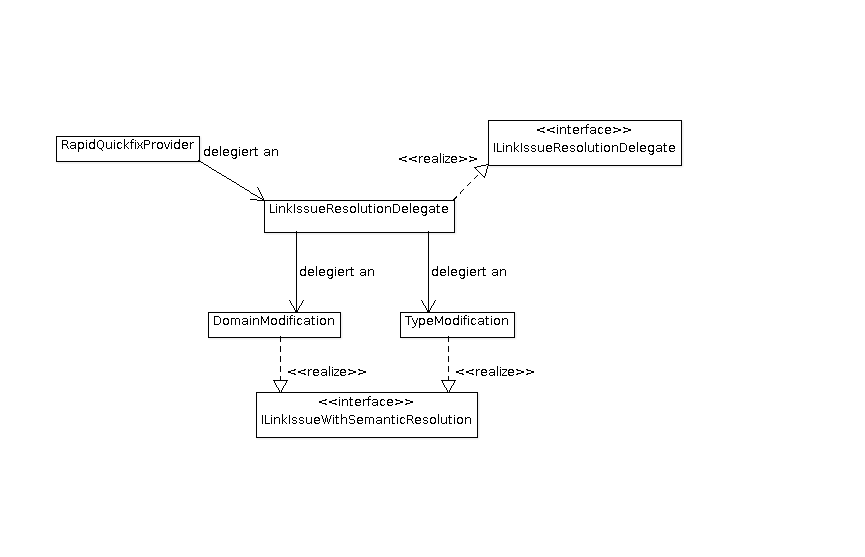
\includegraphics[height=300px]{diagramme/link-issue-resolution.png}
		\caption{Delegierung von Quickfixes}
		\label{fig:link-issue-resolution}
\end{figure}\\
Auf die Quickfixes kann innerhalb des Eclipse-Texteditor mit der Tastenkombination \textit{Strg+1} zugegriffen werden.
\subsection{Documentation Provider}
In Java-Projekten von Eclipse wird beim Überfahren eines Elements mit dem Cursor der JavaDoc-Kommentar der Klasse, des Attributs oder der Methode angezeigt.
Um den Benutzer der DSL ebenfalls die Möglichkeit an die Hand zu geben, sich Informationen über referenzierte Elemente anzuzeigen, wurde die Klasse \verb+RapidEObjectDocumentationProvider+ erweitert. Die darin enthaltene Methode \verb+getDocumentation(EObject eObject)+ wird immer aufgerufen, sobald mit dem Cursor über ein beliebiges Element innerhalb der DSL gefahren wird. Sollte es sich bei dem Methodenparameter \textit{eObject} um eine Instanz einer Domäne, eines Attributs oder eines Prozesses handeln, wird per Java Reflection-Mecha\-nis\-mus überprüft, ob die Eigenschaft \textit{label} oder \textit{description} gesetzt ist. Aus diesen beiden Eigenschaften wird dann die Hover-Dokumentation für das Element innerhalb von Eclipse erzeugt, wie es in Grafik \ref{fig:documentation-provider} zu sehen ist.
\begin{figure}[h]
	\centering
		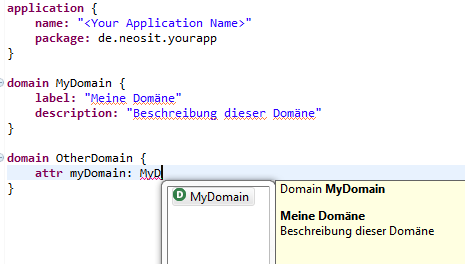
\includegraphics[height=200px]{img/documentation-provider.png}
		\caption{Die vom Documentation Provider erzeugte Dokumentation innerhalb der Umgebung}
		\label{fig:documentation-provider}
\end{figure}\\
\subsection{Outline View}
Unter der Outline View versteht man in Eclipse eine Übersicht über die wichtigsten Elemente innerhalb einer Datei. In Java-Dateien werden beispielsweise alle Attribute, Methoden, Enumerationen und änhliches in einer Baumstruktur aufgelistet, so dass schnell zu den pass\-en\-den Stellen innerhalb des Quellcodes navigiert werden kann.
Xtext erzeugt ebenfalls eine Outline View, die in der Klasse \texttt{RapidOutlineTreeProvider} hinterlegt ist. Die Klasse erbt von \texttt{DefaultOutlineTreeProvider}, die wiederum die Basisfunktionalität für die Erzeugung der Baumstruktur enthält. Die Standardansicht listet alle Schlüssel\-wörter innerhalb der DSL hierarchisch auf. Da diese Ansicht allerdings für den Benutzer sehr un\-über\-sichtlich ist, wurden die Outline View so angepasst, dass logisch zusammenhängende Elemente der DSL gruppiert werden. Um die Darstellung aufzuwerten, wurden innerhalb der \texttt{RapidLabelProvider} für jedes Element, für das ein Icon hinterlegt, die passenden Dateinamen an\-ge\-geben. Das Ergebnis ist in der Grafik \ref{fig:outline-view} zu sehen.
\begin{figure}[h]
	\centering
		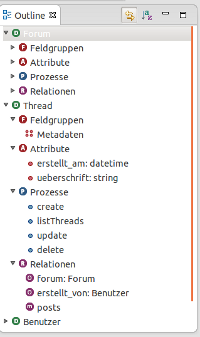
\includegraphics[height=200px]{img/outline-view.png}
		\caption{Outline View für Rapid innerhalb von Eclipse}
		\label{fig:outline-view}
\end{figure}
\subsection{Tests}
Wie auch bei der Erstellung des  Metamodells wurden die Anpassungen der Features mit Unittests abgesichert. Die Tests wurden dabei in der Sprache Xtend geschrieben, so dass Multiline-Strings verfügbar waren. Je nach Komplexität des Testfalls wurden Text-Fixtures entweder in eine eigenständige Datei ausgelagert oder durch Multiline-Strings abgebildet.
Xtext bietet einen eigenen Runner für JUnit an. Außerdem existieren einige Hilfeklassen, mit denen unter anderem die Validatoren auf einfache Weise getestet werden können.
Der Aufbau einer Test\-klasse ähnelt sich dabei:
\begin{verbatim}
@InjectWith(typeof(RapidInjectorProvider))
@RunWith(typeof(XtextRunner))
class RapidDslTest extends AbstractXtextTests {
    @Inject extension ParseHelper<Model>
	
    @Inject extension AnnotationUtil
	
    override setUp() {
        super.setUp();
        with(typeof(de.ckl.rapid.RapidStandaloneSetup));
    }

    @Test
    def enumsCanBeParsed() {
        var rs = '''
enum TestEnum [
    VAL1,
    VAL2,
    VAL3=3
]
'''.parse();

        var enum = rs.enums.head
        assertEquals("TestEnum", enum.name);
   }
}
\end{verbatim}
Mit der Annotation \verb+@Inject+ wird eine Instanz der Klasse \verb+ParseHelper+ injiziert und deren Methoden als Extension Methods für bestehende Klassen verfügbar gemacht.
Mit \verb+@Test+ werden definiert, dass JUnit diese Methode überprüft. Die Extension Method \verb+parse()+ wandelt den Multiline-String in das Ecore-Modell um. Schließlich wird mit der statisch importierten Methode \verb+assertEquals+ der Soll- und Istwert verglichen.
\section{Unterstützung von mehreren Generatoren}
Die langfristige Strategie für Rapid ist, dass sie als Grundlage für die unter Kapitel \ref{sec:verbesserung} beschriebenen Verbesserungen dient.
Die Architektur von Rapid soll dabei zwei Ideen folgen:
\begin{itemize}
	\item \emph{Als Anwender möchte ich dediziert auswählen können, welche Generatoren ich aktiviere.}\\ Ein Webdesigner benötigt keine Function Point-Analyse oder einen Code-Generator für PHP, sondern möchte sich auf das Mocking der Anwendung konzentrieren.
	\item \emph{Als Entwickler möchte ich auf einfache Art und Weise Rapid als DSL Grundlage nutzen und dafür mein eigenen Code-Generator schreiben können.}\\
	Rapid stellt das Grundgerüst für eine DSL zur Verfügung. Anwender, die zum Beispiel Applikationen in Ruby oder Python entwickeln möchten oder müssen, möchten Rapid als Basis nutzen und dafür einen Generator schreiben können.
\end{itemize}
Xtext ist darauf ausgerichtet, dass es zu einer DSL genau einen Generator gibt. Es ist nicht vorgesehen, dass mehrere Generatoren angesprochen werden können. Natürlich könnte der Generator an weitere Generatoren delegieren - die Aufgabe eines Generators ist dabei aber nicht mehr gegeben. Um nun mehrere Generatoren nutzen zu können, muss der Builder Participant erweitert werden. Dies wird im folgenden Kapitel beschrieben.
\subsection{Implementierung eines Builder Participants}
Xtext bietet den Extension Point \emph{org.eclipse.xtext.builder.participant} an. Jedes Klasse, dass diesen Extension Point benutzen will, muss das Interface\\ \verb+IXtextBuilderParticipant+\footnote{org.eclipse.xtext.builder.IXtextBuilderParticipant} implementieren.
Sobald ein Build angestoßen wird, zum Beispiel nach dem Speichern der DSL-Ausprägung, werden alle registrierten Projekt-Builder für die Nature des Projekts ausgeführt. Xtext registriert dabei für Xtext-Natures die Klasse \verb+XtextBuilder+\footnote{org.eclipse.xtext.builder.impl.XtextBuilder}. Die Methode \verb+doBuild(...)+ delegiert letztendlich die Ausführung des Buildprozesses an die Klasse\\
\verb+RegistryBuilderParticipant+\footnote{org.eclipse.xtext.builder.impl.RegistryBuilderParticipant} weiter. Diese liest über die \verb+ExtensionRegistry+ alle Builder aus, die für den Extension Point \emph{org.eclipse.xtext.builder.participant} registriert sind und startet für jeden Participant den Buildprozess.
\\
\\
Innerhalb der \emph{de.ckl.rapid.ui/plugin.xml} ist standardmäßig eingetragen, dass der Extension Point \emph{org.eclipse.xtext.builder.participant} genutzt wird. Die genaue Bin\-dung ist in der \emph{plugin.xml} nicht hinterlegt, sondern nur, dass die Factory\\
\texttt{RapidExecutableExtensionFactory}\footnote{de.ckl.rapid.ui.RapidExecutableExtensionFactory} sich um die Bereitstellung einer solchen Extension kümmert. \verb+RapidExecutableExtensionFactory+ liefert anhand des ge\-bun\-denen Interface-Namens die zugehörige Instanz, die in der Guice-Konfiguration hinterlegt ist.
\\
\\
Zuerst wurde die \verb+MultipleBuilderParticipant+\footnote{de.ckl.rapid.ui.builder.MultipleBuilderParticipant} erstellt, die von \verb+BuilderParticipant+\footnote{org.eclipse.xtext.builder.BuilderParticipant} erbt. \verb+BuilderParticipant+ implementiert das Interface \verb+IXtextBuilderParticipant+ und wird in der \verb+AbstractRapidUiModule+ standardmäßig über Guice an das Interface gebunden.
Damit nun der eigene \verb+MultipleBuilderParticipant+ aufgerufen wird, wurde in der \verb+RapidUiModule+ die Methode \verb+bindIXtextBuilderParticipant()+ überschrieben und die Bindung des Interfaces \verb+IXtextBuilderParticipant+ an die Klasse \verb+MultipleBuilderParticipant+ definiert.
\\
\\
Die einfachste Möglichkeit zum Ausführen eigener Generatoren war nun das Überschreiben der Methode  \verb+handleChangedContents(...)+ innerhalb des\\
\verb+MultipleBuilderParticipant+.
Damit sich neue Artefakt-Generatoren für die DSL registrieren können, wurde in der \text{plugin.xml} ein eigener Extension Point namens \verb+extensionpoint.generator+ innerhalb des Plug-ins \textit{de.ckl.rapid.ui} eingeführt. Jede zu registrierende Extension muss dabei das Interface \verb+IArtifactGenerator+ implementieren.
Die Methode \verb+handleChangedContents(...)+ iteriert über alle registrierten und aktivierten Artefakt-Generatoren und führt diese sequenziell aus. Im UML-Diagramm \ref{fig:builder-participant} ist die Beziehung zwischen den Klassen noch einmal dargestllt.
\begin{figure}[h]
	\centering
		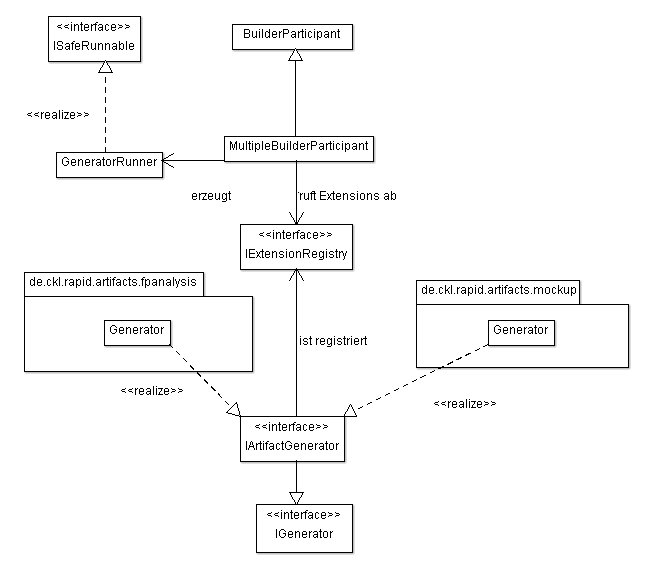
\includegraphics[width=400px]{diagramme/builder-participant.png}
		\caption{Mehrere Generatoren mit der Klasse MultipleBuilderParticipant ansteuern}
		\label{fig:builder-participant}
\end{figure}
\subsection{Auswahl der zu nutzenden Generatoren}
Jeder Anwender sollte die Möglichkeit besitzen, einzelne Artefaktgeneratoren für das Projekt zu aktivieren oder deaktivieren. Aus diesem Grund wurde eine neue Property Page eingeführt. Property Pages werden dargestellt, wenn innerhalb der Eclipse-Umgebung die Einstellungen eines Projekts mit Rechtsklick \textit{Project $\rightarrow$ Properties} oder Tastaturkürzel Alt+Enter aufgerufen werden und beinhalten Konfigurationseinstellungen für ein Projekt.
In der \emph{plugin.xml} wurde dazu der Extension Point \verb+org.eclipse.ui.propertyPages+ genutzt, um eine neue Property Page innerhalb des Abschnitts "Rapid" hinzuzufügen. Die entwickelte Klasse \verb+RapidPropertyPage+ erzeugt dabei mit SWT eine einfache Tabellenansicht der verfügbaren Plug-ins, die im Extension Point \texttt{extensionpoint.generator}\footnote{de.ckl.rapid.ui.extensionpoint.generator} registriert sind. Durch eine Checkbox lässt sich der jeweilige Artefakt-Generator aktivieren bzw. deaktivieren. Sobald der Anwender die Einstellungen speichert, werden die Einstellungen in der Datei \emph{.settings/de.ckl.rapid.ui} persistiert. Die Grafik \ref{fig:property-page-artifact-generators} zeigt die Auswahl der Artefakt-Generatoren innerhalb von Eclipse.
\begin{figure}[h]
	\centering
		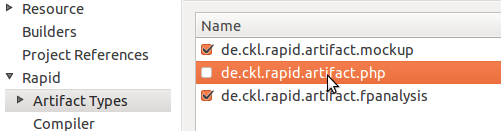
\includegraphics[width=400px]{img/property-page-artifact-generators.png}
		\caption{\label{fig:property-page-artifact-generators}Property Page zur Auswahl der zu aktivierenden Generatoren}
\end{figure}

\section{Erstellen der Generatoren}
Mit der Bereitstellung des Extension Points \texttt{extensionpoint.generator} war die Grundlage geschaffen, damit sich nun beliebige Generatoren in den Build-Prozess der DSL einklinken konnten. Jeder Artefakt-Generator ist dabei ein eigenes Eclipse Plug-in und kann unabhängig von anderen Generatoren ausgeliefert werden. Neue Generatoren können von Entwicklern so unabhängig entwickelt werden.

Um einen neuen Generator zu erzeugen, muss ein neues Eclipse-Plug-in generiert werden. Generatoren sollten dabei innerhalb des Namespaces \verb+de.ckl.rapid.artifact+ liegen.
Nach der Generierung des Plug-in-Grundgerüsts muss in der \emph{plugin.xml} der Extension Point zur Registrierung dieses Generators angesprochen werden:
\begin{verbatim}
   <extension
         point="de.ckl.rapid.ui.extensionpoint.generator">
      <client
          class="de.ckl.rapid.artifact.mockup\
          .GeneratorExtensionFactory:de.ckl.rapid.artifact\
          .mockup.generator.Generator">
      </client>
   </extension>
\end{verbatim}
Da die Plug-ins ebenfalls mit Guice entwickelt werden sollten, muss für jedes Plug-in eine eigene Extension Factory geschrieben werden. Dies ist nötig, da die Zugriffsbeschränkungen für Klassen zwischen den OSGi-Modulen keine weitere Abstrahierung erlaubt.
Die Extension Factory kann dabei folgendermaßen aussehen:
\begin{verbatim}
public class GeneratorExtensionFactory 
    extends RapidExecutableExtensionFactory {
    @Override
    public Bundle getBundle() {
        return FrameworkUtil.getBundle(\
            GeneratorExtensionFactory.class);	
    }

    private Injector generatorInjector;

    public Injector getInjector() {
        if (generatorInjector == null) {
            generatorInjector = super.getInjector()\
            .createChildInjector(
                new GeneratorModule()
            );
        }

        return generatorInjector;
    }
}\end{verbatim}
Wichtig ist, dass die Methode \texttt{RapidExecutableExtensionFactory.getBundle()} überschrieben wird und das ggw. Plug-in zurückliefert. Die Methode \texttt{getInjector()} wird nur benötigt, wenn ein eigenes Guice-Modul benutzt wird. Solch ein Modul könnte z.B. sein:
\begin{verbatim}
public class GeneratorModule extends AbstractGenericModule {
    public Bundle bindBundle() {
        return FrameworkUtil.getBundle(GeneratorModule.class);
    }

    public Class<? extends IJarResourceProvider>\
        bindResourceProvider() {
        return JarResourceProvider.class;
    }
}
\end{verbatim}
Da der Aufbau eines Artefakt-Generators recht ähnlich ist, bietet sich hier eine eigene kleine DSL an, um die Infrastruktur dafür zu erzeugen.
\subsection{Mocking}
Der erste Schritt für den Mocking-Generator bestand darin, dass mit Hilfe von Twitter Bootstrap ein Dummy-Layout erstellt wurde, wie der spätere Mockup aussehen sollte. Twitter Bootstrap bot sich als Framework an, da viele CSS-Klassen bereits vordefiniert sind. Für Softwareentwickler ohne Erfahrungen im Frontenddesign ist dies ein unschätzbarer Vorteil.
Der Mockup wurde danach in eine Xtend-Klasse transformiert, die das Interface \verb+IArtifactGenerator+ implementierte und später in der \emph{plugin.xml} an den Extension Point gebunden wurde.
Im Anschluss an die Entwicklung des Code-Generators folgte die Implementierung der Property Page. Mit dieser können für den Generator folgende Einstellungen gesetzt werden:
\begin{itemize}
	\item Das Ausgabeverzeichnis lässt sich unterhalb des Ordners \emph{src-gen} definieren.
	\item Es existiert die Option, dass transiente Domains nicht in den Mockup übernommen werden, d.h. sie werden in der Navigation nicht angezeigt.
	\item Der Style für die zu generierende DSL konnte ausgewählt werden.
\end{itemize}
Dank der Erfahrungen, die mit der Property Page des Plug-ins zur Aktivierung der Artefakt-Generatoren gemacht worden sind, konnte die Implementierung ebenfalls schnell umgesetzt werden. Die Vorgehensweise hat sich dabei als sehr eingängig erwiesen und besitzt eine klare Struktur.
\\
\\
Die schwierigste Aufgabe dieses Generators bestand darin, die Auswahl der Styles zu implementieren.
Styles sollen dazu dienen, dass ein Mockup auf die Bedürfnisse von Kunden zugeschnitten ist, mit denen man öfter zusammenarbeitet. Ein Webdesigner kann z.B. ein Style namens "NeosIT" definieren, der für alle Projekte des Unternehmens genutzt werden kann.
Nach einigen Überlegungen wurde folgende Implementierung vorgenommen:
\begin{itemize}
	\item Im Ordner \emph{resource/assets} befinden sich alle Dateien, die unabhängig vom gewählten Style immer mit rekursiv in das Ausgabeverzeichnis kopiert werden.
	\item Alle Ordner unterhalb von \emph{resource/styles} können innerhalb der Property Page ausgewählt werden. Beim Speichern wird der Inhalt des Unterordners rekursiv in das Ausgabeverzeichnis kopiert. Bestehende Dateien könnten damit überschrieben werden.
	\item Während des Generierungsprozesses werden zuerst die Dateien kopiert. Der Artefaktgenerator überprüft nach dem Kopiervorgang, welche Dateien in welchem Ordner vorhanden sind und generiert HTML-Tags für die JavaScript- und CSS-Dateien automatisch.
\end{itemize}
Zu beachten war, dass ein Plug-in in aller Regel als ZIP-Datei vorliegt. Das rekursive Kopieren von Verzeichnen aus diesem komprimierten Archiv in ein Projektverzeichnis wurde im Interface \verb+IJarResourceProvider+ definiert und in \verb+JarResourceProvider+ implementiert.
\\
\\
Als Feature für die Mocking-Ansicht wurde mit Hilfe der JavaScript-Klassen  \emph{jQuery Visualize}\footnote{http://filamentgroup.com/lab/update\_to\_jquery\_visualize\_accessible\_charts\_with\_html5\_from\_designing\_with/} und \emph{handsontable}\footnote{http://handsontable.com/} eine editierbare Chart View eingebaut.
Anhand der in der DSL hinterlegten Beispieldaten über das Schlüsselwort \verb+examples+ wird eine Tabelle hinterlegt, die sich in der generierten Ansicht editieren lässt. Das erzeugte Chart wird dabei sofort aktualisiert. Dieses Feature ist für die Entwickler interessant, da die NeosIT in erster Linie Management-Reporting-Systeme entwickelt, bei denen Charts eine wichtige Rolle spielen.
Folgende DSL-Definition ergibt die in der Grafik \ref{fig:editable-chart-table.png} hinterlegte, editierbare Tabelle mit Chart:
\begin{verbatim}
domain Bericht {
    attr wert1: integer {
        examples: ["2", "5", "7"]
    }
    attr wert2: integer {
        examples: ["10", "9", "2"]
    }
    attr wert3: integer {
        examples: ["4", "2", "9"]
    }
    
    process viewGesamtSumme {
        label: "Gesamtsumme aller Werte im Bericht"
        view: statistic [
            self.wert1,
            self.wert2,
            self.wert3
        ]
    }
}
\end{verbatim}
\begin{figure}[h]
	\centering
		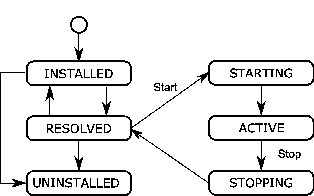
\includegraphics[width=300px]{img/editable-chart-table.png}
		\caption{Editierbares Chart innerhalb des Mockups}
		\label{fig:editable-chart-table.png}
\end{figure}

\subsection{Function Point-Analyse}
Mit der Fertigstellung des Mocking-Generators konnten viele gewonnene Erkenntnisse und Best Practices direkt in den zweiten Generator zum automatischen Erstellen einer Function Point-Analyse (FPA) einfließen.
\\
\\ 
Am Anfang stand die Entscheidung, in welchem Format die FPA erstellt werden sollte. Die einfachste Möglichkeit bestand in der Erstellung einer CSV-Datei, die alle berechneten Werte enthielt. Allerdings wäre die Nachvollziehbarkeit der Berechnung nicht mehr gegeben, da nur noch die Ergebnisse exportiert werden würden. Beim Export der kompletten Datensätze ist es wiederum nötig, dass eine spezielle Excel-Datei existiert, die mit Hilfe von Makros die Analyse auf Basis der CSV-Datei durchführt. Eine zweite Möglichkeit wäre die direkte Generierung einer Excel-Datei mit Hilfe des Frameworks Apache POI\footnote{http://poi.apache.org/} gewesen. Aus Zeitgründen wurde davon abgesehen und schließlich wurde mit Hilfe von JavaScript/jQuery eine kleinere Webanwendung erstellt, die die Analyse anhand der Ausgangsdaten automatisiert durchführt und anzeigt. Weiterhin wurde eine Funktionalität implementiert, mit der man die Einflussfaktoren dynamisch ändern und sich die Ergebnisse ansehen kann.
\\
\\
Die reine Analyse der DSL erfolgt durch ein einfaches Iterieren über die Elemente der DSL. Zuerst werden alle Domänen analysiert:
\begin{itemize}
	\item Domänen, die in der DSL mit  \textit{@ExternalService} annotiert worden sind, werden als External Logical File (ELF) angesehen. Alle anderen Domänen hingegen als Internal Logical File (ILF).
	\item Feldgruppen, die mit \texttt{fieldgroup} innerhalb von Domänen definiert worden sind, werden als Referenced Element Types (RET) beziehungsweise File Types Reference (FTR) gezählt.
	\item Attribute und \texttt{has-many}-Referenzen innerhalb einer Domäne werden als Data Element Type (DET) angesehen.
\end{itemize}
Im zweiten Schritt werden alle Prozesse innerhalb von Domänen überprüft:
\begin{itemize}
	\item Je nach \texttt{view} wird der Prozess als Inquiry, Input oder Output gewertet. Über Annotationen \footnote{siehe \ref{sec:annotationen}} kann der Typ des Functionpoints geändert werden.
	\item Für jede \texttt{view} können die anzuzeigenden Attribute definiert werden. Werden keine Attribute spezifiziert, werden alle Attribute angezeigt. Jedes anzuzeigende Attribut wird als DET gezählt. 
\end{itemize}
Aus diesen Informationen wird eine einfache HTML-Tabelle mit den ungewichteten Function Points generiert. Zusätzlich werden die für das Projekt definierten Komplexitätskriterien ausgelesen und in einer weiteren Tabelle hinterlegt.
Die Berechnung der gewichteten Function Points anhand der Komplexitätskriterien erfolgt durch einfaches JavaScript, die beispielhafte Ausgabe für die Forumsapplikation aus dem Diagramm \ref{fig:beispiel-applikation} ist in der Grafik \ref{fig:fpa-ergebnis} zu sehen. Die Grafik \ref{fig:fpa-ablauf} stellt die Nutzung des Generators für die Function Point-Analyse noch einmal dar.
\begin{figure}[h!]
	\centering
		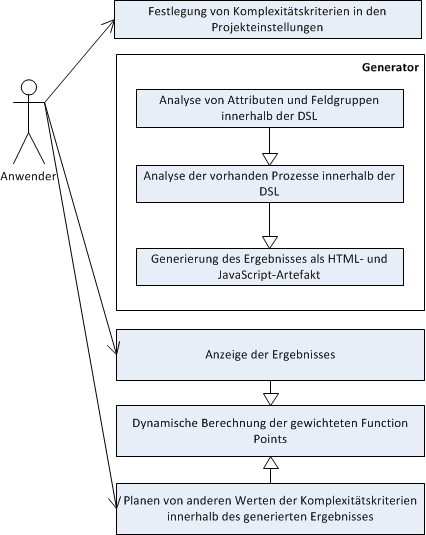
\includegraphics[width=250px]{diagramme/fpa-ablauf.png}
		\caption{Nutzung der Function Point-Analyse}
		\label{fig:fpa-ablauf}
\end{figure}
\begin{figure}[h!]
	\centering
		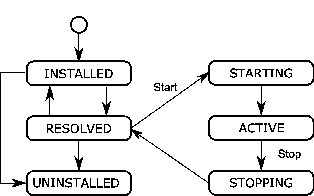
\includegraphics[width=420px]{img/fpa.png}
		\caption{Ausgabe der Function Point-Analyse für die Forumsapplikation}
		\label{fig:fpa-ergebnis}
\end{figure}
\label{sec:annotationen}
\section{Annotationen}
Da die Grammatik von Rapid fest definiert ist, können Entwickler die DSL nicht einfach um eigene Funktionalitäten erweitern. Beispielsweise entstand während der ersten Testphase die Anforderung, dass man bei der Definition der Prozesse hinterlegen kann, um welchen Functiontype (Inquiry, Input, Output) es sich handelt. Der Generator zur Function Point-Analyse sollte damit beeinflusst werden.
Der erste Ansatz bestand darin, innerhalb der Rapid-Grammatik ein neues Element namens \texttt{functiontype} zu hinterlegen.
Allerdings entstehen damit mehrere Probleme: Bei jeder Spracherweiterung muss die Kern-Grammatik angepasst werden. Dies setzt voraus, dass der Entwickler Xtext und ANTLR kennt. Außerdem wird die Grammatik durch diese Erweiterungen verschmutzt, da Rapid nur auf die Modellierung des Datenmodells und der Prozesse ausgelegt ist und über spezifische Eigenheiten der Generatoren keine Kenntnis haben soll.
In Java und C\# werden Metainformationen, wie es z.B. der Functiontype ist, in so genannten Annotationen \cite{annotations} oder Attributen \cite{attributes} hinterlegt. Xtext bietet die Möglichkeit, dass die eigene Grammatik auf Sprachelemente der JVM zugreifen kann. Dieses Feature wurde genutzt, um in Rapid auf Java basierte Annotationen zu integrieren. Entwickler können nun innerhalb ihres Generatores eigene Annotationen in Java definieren, die in der DSL und den Generatoren zur Verfügung stehen. Rapid wird somit von außen erweitert, ohne dass der Kern von diesen Erweiterungen Kenntnis nimmt.
Die Grammatik wurde folgendermaßen umdefiniert:
\begin{verbatim}
grammar de.ckl.rapid.Rapid with 
    org.eclipse.xtext.xbase.annotations.XbaseWithAnnotations

generate rapid"http://www.schakko.de/Rapid"
 
import "http://www.eclipse.org/xtext/common/JavaVMTypes" as types
import "http://www.eclipse.org/Xtext/Xbase/XAnnotations"
// ...
Domain:
    (annotations+=XAnnotation)*
    'domain' name=ID '{'
    // ...
    '}';
	
Attribute:
    (annotations+=XAnnotation)*
    'attr' name=ID ':' dataType=(OptionableDataType)
    // ...
;

Process:
    (annotations+=XAnnotation)*
    'process' name=ID ('{'
    // ...
;	
\end{verbatim}
Mit Hilfe der ersten Zeile \verb+...XBaseWithAnnotations+ wird das Element \verb+XAnnoation+ verfügbar gemacht. Jede Domäne, Attribut, Prozess oder Referenz kann mit beliebig vielen Annotationen ausgezeichnet werden. Innerhalb der \verb+GenerateRapid.mwe2+ musste das Backtracking in ANTLR aktiviert werden, da sonst zwischen den Annotationen innerhalb einer Domäne nicht hätte unterschieden werden können:
\begin{verbatim}
    fragment = parser.antlr.XtextAntlrGeneratorFragment {
        options = {
            backtrack = true
        }
    }
\end{verbatim}
Für das Scoping wurde ein zusätzlicher Provider erstellt, der von der Klasse \verb+XbaseWithAnnotationsScopeProvider+\footnote{org.eclipse.xtext.xbase.annotations.scoping.XbaseWithAnnotationsScopeProvider} erbt. Dieser Provider unterstützt das Scoping für JVM-Elemente, wie es innerhalb der JDT verfügbar ist und bekommt einen weiteren Provider injiziert, der die deklarative Definition der Scopes aus Kapitel \ref{subsec:scoping} enthält. Dieses Vorgehen war nötig, da der \verb+XbaseWithAnnotationsScopeProvider+ keine deklarativen Scopes unterstützt. Sobald kein passender JVM-Typ gefunden wird, delegiert dieser an den deklarativen Scope-Provider weiter.
Über einen zusätzlichen Validator wird definiert, welche Annotationen innerhalb der DSL genutzt werden dürfen. Jede zusätzliche Annotation muss dabei mit mindestens einem der Annotationen \verb+@Attribute+, \verb+@Domain+, \verb+@HasManyReference+ oder \verb+Process+ ausgezeichnet sein.
Innerhalb der DSL kann über 
\begin{verbatim}
    @UseFunctionpointType(FunctionpointType::EXTERNAL_INPUT)
    process mein_prozess {
        view: edit
    }
\end{verbatim}
der Typ spezifiziert werden.
Der Generator überprüft während des Iterierens über das Modell, ob die Annotation vorhanden ist und reagiert dementsprechend darauf.
\chapter{Fazit}
Mit dieser Bachelorthesis wurde der Grundstein für die Integration von Xtext in den bestehenden Softwareentwicklungsprozess bei der NeosIT GmbH gelegt. Die definierte Grammatik der DSL namens Rapid erlaubt es auf einfache Art und Weise Kundenanforderungen zu beschreiben. Die Grammatik ist dabei auf technische Belange ausgerichtet und wird zur Generierung von beliebigen Artefakten benutzt werden.
Die von Xtext generierten Plug-ins wurden dabei so erweitert, dass ein weiterer Extension Point in Eclipse bereitgestellt wurde. 
Die beiden erstellten Generatoren nutzen diesen Extension Point um ihre Artefakte zu generieren. Einerseits erstellt der Generator für das Mocking eine beispielhafte Anwendungsoberfläche, andererseits unterstützt der Generator zur Function Point-Analyse aktiv den Planungsprozess.
\\
Damit die DSL von den Anwender effizient benutzt werden kann, wurden die von Eclipse bzw. Xtext bereitgestellten Features wie z.B. Outline Views, Validierung und Scoping implementiert. Um Abhängigkeiten zwischen den Generatoren und der DSL zu eliminieren, wurde der Support für Annotationen in die DSL und die Scoping Provider integriert. Diese Entscheidung trug besonders dazu bei, dass in der nachfolgenden Betaphase neue Funktionaliäten recht einfach umgesetzt werden konnten.
\\Die Vorstellung der DSL und den damit einhergehenden Möglichkeiten wurde von den Mitarbeitern sehr interessiert aufgenommen. Nach einer kurzen Einführung wurden die bisherigen Projekte innerhalb weniger Stunden in die Sprache von Rapid transformiert. Die erstellten Function Point-Analysen flossen zum direkten Vergleich in das unternehmensinterne Wiki ein. Die Ergebnisse dienen als Grundlage für zukünftige Planungsentscheidungen.
Weiterhin entstanden von den Kollegen innerhalb von kurzer Zeit weitere Generatoren, um beispielsweise anhand der DSL die Schemadefinition für NHibernate zu erzeugen oder mit Spring Roo automatisch Applikationen zu generieren. Die in dieser Arbeit entstandenen Generatoren dienten dabei als Vorlage und Dokumentation. Während der Implementierung neuer Generatoren wurden aufgetretene Fehler und Verbesserungsvorschläge direkt umgesetzt.
Weiterhin wurde durch die in dieser Arbeit gemachten Erfahrungen mit Xtext vom Autor innerhalb von zwei Stunden eine weitere DSL entwickelt, mit der sich einfache Expertensysteme abbilden lassen. Diese DSL wird bereits ebenfalls produktiv eingesetzt.
\\
\\
Mit der Einarbeitung in Xtext haben sich viele neue Möglichkeiten zur Verbesserung und Automatisierung aufgetan. Mit Rapid ist ein stabiles und einfach erweiterbares Framework entstanden. Das Ökosystem von Generatoren rund um die DSL unterstützt bereits jetzt erfolgreich den Softwareentwicklungsprozess der NeosIT.
\chapter{Ausblick}
In Kapitel \ref{sec:verbesserung} wurden bereits einige Ideen für Artefaktgeneratoren genannt. Die momentane Ausrichtung der NeosIT auf die Entwicklung in C\# macht es nötig, dass der sich bereits im Einsatz befindende Xtext-C\#-Generator in Rapid abgebildet wird. Hier wäre eine Wizard-Erweiterung für Eclipse sinnvoll, mit der sich das Grundgerüst von neuen Artefaktgeneratoren für Rapid recht einfach erstellen ließ. Diese Idee kam während der Umsetzung des Generators für die Function Point Analyse, da sich die Struktur der Generatoren doch ähnelt aber nicht weiter abstrahiert werden kann.
Auch zu überlegen ist die Erzeugung von aufbereiteten POJOs, die von Apache Isis\footnote{Isis steht unter Apache License 2.0 und kann unter http://isis.apache.org heruntergeladen werden.} weiterverarbeitet werden können. Isis ist ein Framework zum Generieren von Prototypen mit verschiedenen Ausgabeformaten, z.B. XML und HTML. Als Basis kommen dabei Java-Technologien zum Einsatz. Rapid könnte mit relativ wenig Aufwand Code für Isis erzeugen, der sofort lauffähig wäre.
\\
Ein wichtiger Punkt ist die Integration von Rapid in den Buildserver. Das Rapid Plug-in und die Generatoren werden momentan noch manuell innerhalb von Eclipse erzeugt. Hier soll in Zukunft der Build automatisiert durch TeamCity erfolgen. Die Plug-ins sollen als Eclipse Update Site zur Verfügung stehen.
% ==========[ An dieser Stelle beginnt der Anhang ]==========

% Anhang
\appendix

% Layout pruefen und Nummerierung anpassen
\leerSeiteAnhang

\chapter*{Eidesstattliche Erklärung}
Hiermit versichere ich, dass die vorliegende Arbeit von mir selbstständig und ohne unerlaubte Hilfe 
angefertigt worden ist, insbesondere dass ich alle Stellen, die wörtlich oder annähernd wörtlich aus 
Veröffentlichungen entnommen sind, durch Zitate als solche gekennzeichnet habe. Ich versichere 
auch, dass die von mir eingereichte schriftliche Version mit der digitalen Version übereinstimmt. 
Weiterhin erkläre ich, dass die Arbeit in gleicher oder ähnlicher Form noch keiner anderen 
Prüfungsbehörde vorgelegen hat. Ich erkläre mich damit einverstanden/nicht einverstanden, dass die 
Arbeit der Öffentlichkeit zugänglich gemacht wird. Ich erkläre mich damit einverstanden, dass die 
Digitalversion dieser Arbeit zwecks Plagiatsprüfung auf die Server externer Anbieter hochgeladen 
werden darf. Die Plagiatsprüfung stellt keine Zurverfügungstellung für die Öffentlichkeit dar.
\\
\\
\\
Datum, Unterschrift
	
% ==========[ Abkuerzungsverzeichnis ]==========

\begin{abkuerzung}\label{abk}

% Bitte achten Sie auf die alphabetische Sortierung!
\abkuerzungEintrag{API}{Application Programming Interface}
\abkuerzungEintrag{CRUD}{Create, Read, Update, Delete}
\abkuerzungEintrag{CSS}{Cascading Stylesheet}
\abkuerzungEintrag{CSV}{Comma-separated values}
\abkuerzungEintrag{DAL}{Data Access Layer}
\abkuerzungEintrag{DAO}{Data Access Object}
\abkuerzungEintrag{DBMS}{Datenbank Management System}
\abkuerzungEintrag{DDL}{Data Definition Language}
\abkuerzungEintrag{DET}{Data Element Type}
\abkuerzungEintrag{DSL}{Domain Specific Language}
\abkuerzungEintrag{ELF}{External Logical File}
\abkuerzungEintrag{EMF}{Eclipse Modeling Framework}
\abkuerzungEintrag{FTR}{File Type Reference}
\abkuerzungEintrag{FPA}{Function Point-Analyse}
\abkuerzungEintrag{HTML}{Hypertext Markup Language}
\abkuerzungEintrag{IDE}{Integrated Development Environment}
\abkuerzungEintrag{ILF}{Internal Logical File}
\abkuerzungEintrag{JDT}{Java Development Toolkit}
\abkuerzungEintrag{JPA}{Java Persistence API}
\abkuerzungEintrag{JVM}{Java Virtual Machine}
\abkuerzungEintrag{MDA}{Model Driven Architecture}
\abkuerzungEintrag{MWE}{Model Workflow Engine}
\abkuerzungEintrag{PDE}{Plug-in Development Environment}
\abkuerzungEintrag{PDT}{PHP Development Toolkit}
\abkuerzungEintrag{POJO}{Plain Old Java Object}
\abkuerzungEintrag{RET}{Record Element Type}
\abkuerzungEintrag{SCM}{Source Code Management}
\abkuerzungEintrag{SWT}{Standard Widget Toolkit}
\abkuerzungEintrag{TDD}{Test Driven Development}
\abkuerzungEintrag{UML}{Unified Modeling Language}


\end{abkuerzung}



% ==========[ Verzeichnisse ]==========

% Nicht gewuenschte Verzeichnisse koennen auskommentiert werden
% Abbildungsverzeichnis und Tabellenverzeichnis auf einer Seite, da zu wenig Grafiken bzw. Tabellen vorhanden
\listoffigures
\addcontentsline{toc}{chapter}{Abbildungs- und Tabellenverzeichnis}
\begingroup
\let\clearpage\relax
\listoftables
\endgroup



% ==========[ Glossar ]==========

\begin{glossar}\label{glossar}

% Bitte achten Sie auf die alphabetische Sortierung!
\glossarEintrag{Annotation}{Annotationen dienen dazu, Metadaten innerhalb einer Programmiersprache oder DSL zu hinterlegen.}
\glossarEintrag{Artefakt}{Ein Artefakt stellt im Rahmen dieser Arbeit ein oder mehre Quellcodedateien dar, die automatisiert erzeugt worden sind.}
\glossarEintrag{Artefakt-Generator}{Ein Plug-in zur automatisierten Erstellung von Artefakten bzw. Quellcode. Der Generator nutzt dabei das Modell der DSL als Basis.}
\glossarEintrag{Domäne}{Als Domäne wird der Bereich bezeichnet, in dem eine domänenspezifische Sprache eingesetzt wird.}
\glossarEintrag{Eclipse}{Eine Entwicklungsumgebung für Java und andere Programmiersprachen}
\glossarEintrag{Function Point-Analyse}{Methodik, die zur Aufwandsabschätzung von Softwareprojekten angewandt werden kann.}
\glossarEintrag{Lambda-Ausdruck}{Ein Lambda-Ausdruck stellt eine anonyme Funktion dar, die an eine Methode übergeben werden kann.}
\glossarEintrag{Mockup}{Beispielhafte Darstellung einer Anwendung ohne oder mit wenig Funktionalität.}
\glossarEintrag{Modell}{Das Modell bildet mit Hilfe der DSL die Anforderungen einer Domäne in einer textuellen Form ab.}
\glossarEintrag{transient}{Ein Element (Domäne, Attribut o.ä.), das zur Laufzeit nicht in einer Datenbank persistiert wird.}
\end{glossar}



% ==========[ Literaturverzeichnis ]==========

\nocite{*}
\addcontentsline{toc}{chapter}{Literaturverzeichnis}
\bibliography{wissenschaftlich_arbeiten_latex}



% ==========[ Index ]==========

% Bitte beachten Sie zur Erstellung des Index die Hinweise in der
% beiligenden Anleitung im PDF-Format, da sonst kein Index fuer
% das Dokument erstellt und ausgegeben wird.

% \indexInhalt
% \printindex

\end{document}

